%  LaTeX support: latex@mdpi.com
%  In case you need support, please attach all files that are necessary for compiling as well as the log file, and specify the details of your LaTeX setup (which operating system and LaTeX version / tools you are using).

% You need to save the "mdpi.cls" and "mdpi.bst" files into the same folder as this template file.

%=================================================================
\documentclass[ijgi,article,accept,moreauthors,pdftex,10pt,a4paper]{mdpi} 

%=================================================================
\firstpage{1}
\makeatletter 
\setcounter{page}{\@firstpage} 
\makeatother 
\articlenumber{x}
\doinum{10.3390/------}
\pubvolume{xx}
\pubyear{2016}
\copyrightyear{2016}
\externaleditor{Academic Editors: Marguerite Madden and Wolfgang Kainz}
\history{Received: 15 August 2016; Accepted: 28 September 2016; Published: date}
%------------------------------------------------------------------
% The following line should be uncommented if the LaTeX file is uploaded to arXiv.org
%\pdfoutput=1

%=================================================================
% Add packages and commands here. The following packages are loaded in our class file: fontenc, calc, indentfirst, fancyhdr, graphicx, lastpage, ifthen, lineno, float, amsmath, setspace, enumitem, mathpazo, booktabs, titlesec, etoolbox, amsthm, hyphenat, natbib, hyperref, footmisc, geometry, caption, url, mdframed

%=================================================================

\usepackage{placeins}


%% Please use the following mathematics environments:
 \theoremstyle{mdpi}
 \newcounter{thm}
 \setcounter{thm}{0}
 \newcounter{ex}
 \setcounter{ex}{0}
 \newcounter{re}
 \setcounter{re}{0}

 \newtheorem{Theorem}[thm]{Theorem}
 \newtheorem{Lemma}[thm]{Lemma}
 \newtheorem{Corollary}[thm]{Corollary}
 \newtheorem{Proposition}[thm]{Proposition}

 \theoremstyle{mdpidefinition}
 \newtheorem{Characterization}[thm]{Characterization}
 \newtheorem{Property}[thm]{Property}
 \newtheorem{Problem}[thm]{Problem}
 \newtheorem{Example}[ex]{Example}
 \newtheorem{ExamplesandDefinitions}[ex]{Examples and Definitions}
 \newtheorem{Remark}[re]{Remark}
 \newtheorem{Definition}[thm]{Definition}
%% For proofs, please use the proof environment (the amsthm package is loaded by the MDPI class).

%=================================================================
% Full title of the paper (Capitalized)
%\Title{Exploring multi-scale spatiotemporal Twitter user mobility patterns with a scalable visual-analytics framework}
\Title{Exploring Multi-Scale Spatiotemporal Twitter User Mobility Patterns with a Visual-Analytics Approach}

% Authors, for the paper (add full first names)
\Author{Junjun Yin $^{1,3}$ and Zhenhong Du $^{2,3,*}$}
% Authors, for metadata in PDF
\AuthorNames{Junjun Yin and Zhenhong Du}

% Affiliations / Addresses (Add [1] after \address if there is only one affiliation.)
\address{%
$^{1}$ \quad Department of Geography and Geographic Information Science, University of Illinois at Urbana-Champaign, Urbana, IL 61801, USA; jyn@illinois.edu\\
$^{2}$ \quad Institute of Geographic Information Science, School of Earth Sciences, Zhejiang University, Hangzhou 310028, China; duzhenhong@zju.edu.cn\\
$^{3}$ \quad CyberGIS Center for Advanced Digital and Spatial Studies, University of Illinois at Urbana-Champaign, Urbana, IL 61801, USA}

% Contact information of the corresponding author
\corres{Correspondence: duzhenhong@zju.edu.cn; Tel.: +86-138-1919-2989}

% Current address and/or shared authorship

% Simple summary
%\simplesumm{}

% Abstract (Do not use inserted blank lines, i.e. \\) 
\abstract{Understanding human mobility patterns is of great importance for urban planning, traffic management, and even marketing campaign.
However, the capability of capturing detailed human movements with fine-grained spatial and temporal granularity is still limited.
In this study, we extracted high-resolution mobility data from a collection of over 1.3 billion geo-located Twitter messages.
Regarding the concerns of infringement on individual privacy, such as the mobile phone call records with restricted access, the dataset is collected from publicly accessible Twitter data streams.
In this paper, we employed a visual-analytics approach to studying multi-scale spatiotemporal Twitter user mobility patterns in the contiguous United States during the year 2014.
Our approach included a scalable visual-analytics framework to deliver efficiency and scalability in filtering large volume of geo-located tweets, modeling and extracting Twitter user movements, generating space-time user trajectories, and summarizing multi-scale spatiotemporal user mobility patterns.
We performed a set of statistical analysis to understand Twitter user mobility patterns across multi-level spatial scales and temporal ranges.
In particular, Twitter user mobility patterns measured by the displacements and radius of gyrations of individuals revealed multi-scale or multi-modal Twitter user mobility patterns.
By further studying such mobility patterns in different temporal ranges, we identified both consistency and seasonal fluctuations regarding the distance decay effects in the corresponding mobility patterns.
At the same time, our approach provides a geo-visualization unit with an interactive 3D virtual globe web mapping interface for exploratory geo-visual analytics of the multi-level spatiotemporal Twitter user movements.}

% Keywords
\keyword{Geo-located tweets, mobility patterns, multi-scale spatiotemporal analysis, scalable visual-analytics framework}
\begin{document}

%%%%%%%%%%%%%%%%%%%%%%%%%%%%%%%%%%%%%%%%%%
%% Sections that are not mandatory are listed as such. The section titles given are for Articles. Review papers and other article types have a more flexible structure. 

%% Only for the journal Gels: Please place the Experimental Section after the Conclusions

%%%%%%%%%%%%%%%%%%%%%%%%%%%%%%%%%%%%%%%%%%
\section{Introduction}
Understanding human mobility patterns is of great importance for a broad range of applications from urban planning~\cite{zheng2008understanding}, traffic management~\cite{jiang2009characterizing}, and even the spatial spread of epidemic diseases~\cite{belik2011natural}.
Earlier research efforts relied on low-resolution mobility data to understand human mobility patterns, such as using census records to study human migration patterns~\cite{greenwood1985human}, or delivering questionnaires and asking volunteers to report the track of bank notes to infer human travel patterns~\cite{brockmann2006scaling}.
However, such mobility data do not provide detailed human movements with fine-grained spatial and temporal granularity, which are usually aggregated and therefore are limited to capture mobility patterns of individuals~\cite{gonzalez2008understanding,Jurdak2015}.
In addition to the mobility data collected by GPS trackers~\cite{zheng2008understanding, rhee2011levy} and mobile phone call records~\cite{gonzalez2008understanding,sevtsuk2010does,kung2014exploring}, emerging as a new mobility data source, today's pervasive Location Based Social Media (LBSM) platforms (e.g., Twitter and Foursquare) offer continuous spatial Big Data streams with massive amount of detailed and frequently updated user digital footprints in the form of real-world user trails and footprints~\cite{thatcher2014living}.
A significant advantage of utilizing LBSM data streams as proxies for studying human mobility patterns is the large spatial coverage.
For instance, researchers have used geo-located tweets for studying global mobility patterns~\cite{hawelka2014geo}, which is otherwise impossible for other mobility datasets (e.g., GPS traces and mobile phone call records).
Regarding the concerns of infringement on individual privacy, such as the mobile phone call records with restricted access~\cite{giannotti2008mobility,crampton2014collect,Jurdak2015}, the publicly available LBSM data streams offer unique opportunities for conducting reproducible and comparative scientific findings across different geographic regions.

Many recent studies have adopted LBSM data streams to study human mobility patterns.
For example, they modeled and extracted trajectories of individuals and performed statistical analysis focusing on the distance decay effects in the collective user movements~\cite{gonzalez2008understanding}, which were used to reveal different travel modes~\cite{Jurdak2015}, travel demands~\cite{wu2014intra,hasan2013understanding}, and the impact of social connections~\cite{cho2011friendship}.
These studies have provided strong supports for using LBSM data as proxies for studying mobility patterns of individuals and valuable insights into human mobility dynamics.
However, the variations of movements in different spatial scales and temporal ranges are neglected in these studies, where the measurements of distances are either fixed in a certain time range or to a specific geographic region.
For instances, the examinations on whether there are temporal (e.g., monthly or seasonal) changes within the movements or how the observed mobility patterns vary across different spatial scales (e.g., intra- or inter city or national levels) are lacking.
Such insights are critical to advance our understandings of the collective mobility patterns for various applications, such as examining the mobility patterns across different cities~\cite{noulas2012tale}, the spread patterns of disease~\cite{balcan2009multiscale, tamerius2011global} and touristic activities~\cite{hawelka2014geo}.
On the other hand, while the high-resolution spatiotemporal records from LBSM present unique research opportunities in this direction, the inherited large data volume poses significant data-intensive challenges for developing multi-scale spatiotemporal analysis approaches to dealing with the complexities in filtering movements of individuals, modeling and aggregating user trajectories at multiple spatial and temporal scales~\cite{tsou2015}.

In this paper, we have employed a visual-analytics approach to exploring the Twitter user mobility patterns across multi-level spatial scales and temporal ranges in the continuous United States (i.e., excluding Alaska and Hawaii) during the year 2014.
The mobility data is extracted from over 1.3 billion geo-located Twitter messages (i.e., tweets) from 1st January to 31st December 2014 over North America with over 6 million Twitter users and over 1 TB in file size.
To address the data-intensive challenge embedded in this dataset, we have developed a scalable visual-analytics framework tailored to accommodate large volume of geo-located tweets.
This framework is implemented based on high-performance distributed computing environment using Apache Hadoop (http://hadoop.apache.org/), which is an open source software framework to enable distributed processing of large datasets across computing clusters.
Enabled by this framework, we have performed a set of statistical analysis to understand multi-scale spatiotemporal Twitter user mobility patterns. 
We have modeled the frequency of Twitter users visiting different locations to study the collective user visiting behaviors, where we have identified temporal similarities in the distributions.
In particular, Twitter user mobility patterns measured by user displacements and radius of gyrations of individuals~\cite{gonzalez2008understanding} have revealed different groups of Twitter users with multi-scale or multi-modal mobility patterns and multiple travel modes~\cite{Jurdak2015}.
By further studying such mobility patterns in different temporal ranges, we have identified both consistency and seasonal fluctuations regarding the distance decay effects in the corresponding mobility patterns.
In addition, our approach provides an interactive 3D virtual globe web mapping interface to enable exploratory geo-visual analytics for understanding the detailed Twitter user movement flows within a given spatial scale and time window.

The remainder of this paper is organized as follows.
Section 2 describes the related work in the context of studying mobility patterns using LBSM data, in particular, the geo-located Twitter data.
We focus on research challenges in using visual-analytics methods to enable multi-scale spatiotemporal analysis with massive movement datasets, including data management, multi-level spatiotemporal user trajectory modeling and visualization.
Section 3 details the processes for extracting, aggregating and summarizing multi-level spatiotemporal Twitter user mobility patterns.
Section 4 presents the case study of performing visual-analytics for seeking multi-scale spatiotemporal Twitter mobility patterns in the continuous United States of the year 2014.
Section 5 concludes the paper.

\section{Mobility Patterns in Location Based Social Media data}
\subsection{Geo-located Twitter Data for Studying Large-scale User Movements}
To understand detailed mobility patterns of individuals, the capability to capture human movements with fine-grained spatial and temporal granularity is critical.
In this connection, using GPS trackers tends to produce, to date, the most accurate records of individuals' movements regarding the accuracy of recorded user locations and update frequency~\cite{zheng2008understanding}.
However, such data are often limited in spatial scale (e.g., within a specific city or region) from a small group of people, for example, 226 and 182 volunteers participated in collecting such mobility data in~\cite{rhee2011levy} and~\cite{zheng2010geolife} respectively.
Other than tracking people directly, the vehicle-based GPS traces are often tied to specific vehicles (e.g. taxi), which are only accessible for a certain group of people~\cite{kung2014exploring}. 

Another approach from the literatures for studying human mobility is using mobile phone call data, such as Call Detail Records (CDR), where the locations of mobile users are estimated by cell tower triangulation with an accuracy in the order of kilometers~\cite{gonzalez2008understanding,sevtsuk2010does,kung2014exploring}.
Such a dataset can cover relatively large spatial scale~\cite{becker2013human,sobolevsky2013delineating} (e.g., national level) and a large portion of the population in the study region~\cite{kung2014exploring}.
However, due to the concerns of infringement on individual privacy, mobile phone call data are not publicly accessible at all.
Even such data were obtained in the mentioned studies, they came from various service providers covering different groups of users.
These issues limit the capability for conducting reproducible scientific findings for mobility research, such as validating or extending the existing discoveries.

In this connection, it becomes increasingly popular for researchers to exploit the publicly accessible mobility data captured from today's pervasive Location Based Social Media (LBSM) platforms (e.g., Foursquare and Twitter).
LBSM enables users to attach their current location as a geo-tag to the message they post, which is derived from either the GPS or Wi-Fi positioning with a high position resolution down to 10 meters~\cite{Jurdak2015}.
A Big Data scenario emerges when millions social media users constantly post messages.
In this study, geo-located Twitter data are chosen as a source for studying detailed mobility patterns.
Compared to other LBSM platforms, Twitter is one of the most popular platforms and is been actively used in many countries.
It provides a publicly accessible streaming API for easy data access~\cite{twitterAPI}.
Indeed, many other LBSM data can be collected from the data streams, such as Foursquare check-in data~\cite{cranshaw2012livehoods,hasan2013understanding}.

However, it is worth noting that there are some limitations and complexities in directly using LBSM data for studying human mobility patterns.
For example, comparing to GPS traces, the update frequency of an individual's location varies depending on when a user is posting a new geo-located message or check-in at a new place.
Although geo-located tweets tend to provide geo-locations with high position resolution as aforementioned~\cite{Jurdak2015}, the information regarding the quality of the geo-locations is absent in each tweet.
This will contribute to the uncertainties in calculating the distance of Twitter user movements, especially in densely built environments.   
There is also a potential mismatch regarding the representativeness of the overall population since not all people use social media or send geo-located messages~\cite{kung2014exploring}, the demographic information of the Twitter users cannot be easily identified.
The derived mobility patterns may lead to an over or under-representation of the real-world human mobility patterns.
Many studies started to look into the demographic information of LBSM data, in particular Twitter data~\cite{mitchell2013geography,longley2015geotemporal}.
Although the used methods are still arguable, these issues certainly require us to pose stricter criteria in understanding human mobility patterns using geo-located Twitter data.
On the other hand, geo-located Twitter dataset presents some unique advantages that make it a valuable proxy for studying human mobility patterns.
For example, the high-resolution location information enables to identify multiple travel modes in user mobility patterns~\cite{Jurdak2015}; the large spatial coverage enables to study global mobility patterns~\cite{hawelka2014geo}, which is almost impossible for other mobility datasets.
More importantly, by continuously monitoring the geo-located Twitter data streams with large volume of detailed and frequently updated spatiotemporal records of Twitter users, it offers a great deal of potential for studying mobility patterns of large groups of individuals at different spatial scales (e.g., movements across cities, states or even countries) and temporal gratuity (e.g., weekly, monthly, and seasonal movements), which is one of the motivations for this study.

\subsection{Data-intensive Challenges for Multi-scale Geo-visual Analytics}
Mobility data are essentially a collection of spatiotemporal records of people re-allocating across the geographic space.
To study mobility patterns of individuals, a space-time trajectory of each individual user should be modeled and constructed to quantify the collective movements over space and time.
Based on the extracted space-time trajectories, aforementioned studies are able to perform analysis, such as the measurements of user displacements and radius of gyrations of individuals, to study the mobility dynamics.
Indeed, space-time trajectory is one of the core concepts in H{\"a}gerstrand's time geography to understand the embedded spatiotemporal dynamics~\cite{hagerstrand1985time}, which has provided useful insights to explore movements across different geographical scales and temporal ranges.
For example, a geo-visualization approach was used to study human activity patterns, where user trajectories were mapped in a 3D space ordered by timestamps in the third dimension~\cite{kwan2004geovisualization}.
While such an approach enables visualization of individual trajectories, its capability is limited in dealing with large-volume movement datasets~\cite{andrienko2007designing}.
Instead of directly visualizing an individual user's trajectories, a space-time cube approach was proposed to analyzing and visualizing the collective trajectories.
It provides flexibilities in setting up both spatial scales and temporal ranges, and therefore is used to study mobility patterns across different spatial units (e.g., countries, states, and cities, etc.) and identify the changes over space and time~\cite{maceachren2001research, maceachren2004maps}.
In this regard, visual-analytics methods are proposed to better convey the findings in terms of analyzing and visualizing multi-level spatiotemporal mobility patterns~\cite{andrienko2007designing,andrienko2007visual}.
Visual-analytics methods focus on the synergy of computational and analytical methods to reduce the visual clutter, where aggregation methods are suggested to perform grouping/dividing individual's moving trajectories at different spatial and temporal granularity, e.g., utilizing the space-time cube approach~\cite{andrienko2007designing}.
Employing visual-analytics methods dealing with massive movement datasets is not only beneficial for optimizing visualizations but also provides a great deal of flexibilities for performing statistical analysis in seeking mobility patterns with different level of spatiotemporal details. 

However, in the context of studying mobility patterns using large volume of geo-located Twitter data, the inherited large data volume poses significant data intensive challenges for visual-analytics methods to scale with both the data volume and the computational requirements (e.g., movement extraction and trajectory modeling)~\cite{cao2014scalable}.
In particular, in our study, 1.3 billion geo-located tweets were collected with over 1 TB in file size.
To construct a space-time trajectory of an individual, it is necessary to go through the massive dataset to sort and update the trajectory whenever a new location is found.
Such a task is already computationally demanding, let along breaking the trajectories to construct space-time cube with multiple spatial scale and temporal ranges.
Indeed, developing a multi-scale spatiotemporal analysis approach is identified as one of the research challenges for dealing with social media Big Data~\cite{tsou2015}.
To address the data-intensive challenges, there is a need to develop a scalable visual-analytics framework tailored to accommodate large volume of geo-located tweets for studying multi-level spatiotemporal Twitter user mobility patterns.


\section{Materials and Methods}
\subsection{Geo-located Twitter Data}
Geo-located tweets are tweets appended with an additional geo-tag in the form of a pair of geographical coordinates, which represents the location a tweet was sent at.
In this study, the geo-located tweets were downloaded using the Twitter Streaming API, where we specified a geographical bounding box as an area-of-interest to retrieve all the geo-located tweets that fall within it.
To ensure complete coverage over the continuous United States, we implemented a crawler that selects North America as the initial area-of-interest, where the geographical boundary is specified with lower left (latitude: 5.4, longitude: -167.3) and upper right (latitude: 83.2, longitude: -52.2).
The crawler is constantly running with over 2 million geo-located raw tweets ($\sim$2 GB in size) collected per day.
We have collected more than 1.3 billion geo-located tweets from 1 January to 31 December 2014 with 6,147,430 Twitter users and 1 TB in file size.

In particular, this data collection of the year 2014 was originally used to map the spatial spread of flu in North America during the time period~\cite{padmanabhan2014flumapper}.
As a social media account is not equal to a real person in the physical world~\cite{tsou2015}, to ensure the data quality, the collected raw tweets were further filtered by the following steps: We first removed duplicated messages in the dataset~\cite{black2012twitter}; and then we removed non-human users based on the heuristic of unusual relocating speed discussed in~\cite{hawelka2014geo,Jurdak2015}.
In this case, we adopted the speed limit value as 240 m/s used in~\cite{Jurdak2015}, where we examined all the consecutive locations of each user and excluded those with relocating speed over the limit.
Note that the original location information embedded in each geo-located tweet is given in units of latitude and longitude, the distance is calculated by the great-circle distance between two points on a sphere with the haversine formula.
Finally, we used the geographic boundaries of the continuous United States (excluding Alaska and Hawaii) to further restrict the remaining tweets, where the technical details is presented in the following section. Based on these reinforcements, the dataset contains 1,052,861,000 tweets and 4,559,205 unique users.

\subsection{A scalable visual-analytics framework}
To address the data-intensive challenges, we have developed a scalable visual-analytics framework tailored to accommodate large volume of geo-located tweets for studying multi-level spatiotemporal Twitter user mobility patterns.
The scalable visual-analytics framework consists of two main units: (1) Data processing unit: a distributed computing environment using Apache Hadoop for modeling and extracting Twitter user movements, generating space-time user trajectories, and summarizing the movements at multiple spatiotemporal scales.
(2) Geo-visualization unit: an interactive 3D virtual globe web mapping interface for exploratory geo-visual analytics to understand detailed Twitter user movement flows across different spatial scales and temporal ranges. 

Apache Hadoop combines a distributed file system, namely Hadoop Distributed File System(HDFS)~\cite{shvachko2010hadoop} with MapReduce programming paradigm~\cite{dean2008mapreduce}, which can be applied to a wide range of data-intensive problems.
Our framework benefits from using Hadoop in both data management and processing.
First, since the input data is large it is desirable to store it on multiple machines.
This provides scalability in relation to the growth of data size, where Hadoop can scale to more computing nodes in a cluster to maintain the performance.
Second, by using Hadoop we can parallelize the computational tasks, where MapReduce breaks the entire computation into small tasks and schedule them among different computing nodes, to make the data processing faster and more efficient.
An overall system architecture of the framework is shown in Figure~\ref{fig:overall_archi}.
The details regarding the function and implementation of each unit are presented in the next sections.

\begin{figure}[ht]
\centering
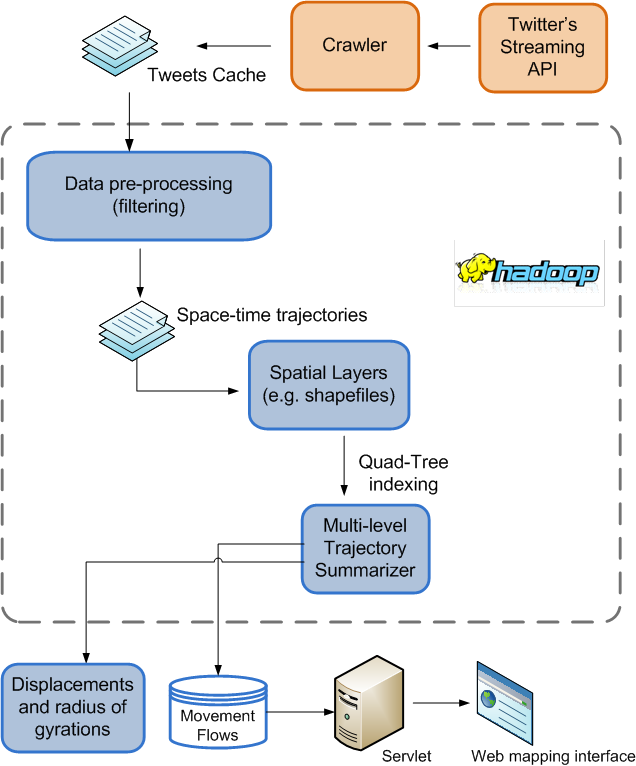
\includegraphics[width=0.55\linewidth]{./figures/Overall_Architecture222}
\caption{The overall system architecture of the framework.}
\label{fig:overall_archi}
\end{figure}
\FloatBarrier

\subsection{Space-time Twitter User Trajectories}
To derive meaningful mobility patterns of individuals, a space-time trajectory of each individual user should be constructed~\cite{hagerstrand1985time}.
Each raw geo-located tweet contains multiple fields of information, such as the created time, country, language code, and location, etc.
To construct a space-time trajectory from the data collection, we are interested in the following fields: \textit{user ID, location, timestamp}, which can be represented by a tuple $\left\langle id, loc, t\right\rangle$, where \textit{id} is a unique string representing a Twitter user's id; \textit{loc} is the recorded location of the message represented as a pair of projected coordinates $\left\langle x, y\right\rangle$;
and \textit{t} is the timestamp of when the message was posted; A Twitter user's space-time trajectory is defined as follows.
\newline

\noindent\textbf{Definition 1. Space-time Twitter user trajectory:} \emph{The space-time trajectory of a Twitter user is defined as a collection of recorded geo-locations in the chronological order (i.e., based on the attached timestamp):} 
\newline

$Trajectory_{user_{id}} \equiv \lbrace \langle id, loc_{1}, t_{1}\rangle, \langle id, loc_{2}, t_{2}\rangle, \langle id, loc_{i}, t_{i}\rangle, ... \langle id, loc_{n}, t_{n}\rangle \rbrace, i = 1, 2, 3...n$
\newline

To remove non-human users based on unusual relocating speed, a user will be removed if the speed between any two consecutive locations in the user's trajectory with $speed$ $(loc_{i} - loc_{i-1}) > $ 240 m/s.
Based on this definition for modeling the space-time Twitter user trajectories, we converted the process of extracting trajectories from the raw geo-located Twitter data as a MapReduce task. Specifically, each mapper utilizes the unique user id as a key to prepares the records that belong to the same user and send them to reducer. Once the reducers receive the $\langle key, value\rangle$ pairs, a Twitter user's space-time trajectory is formed by the sorting the locations in chronological order while considering the speed limit.
\newline

\noindent\textbf{Definition 2. visitation behavior, displacement and radius of gyration:} \emph{As each space-time Twitter user trajectory records all the locations a user has visited, the visitation behavior refers the frequency of a user visiting different locations within a specific time frame.
This metric provides an overall assessment regarding the diversity and similarity in the collective mobility pattern}~\cite{gao2012exploring}.

In particular, the measurements of displacements and radius of gyrations of individuals are two popular metrics to investigate and quantify the distance decay effects in the collective mobility patterns~\cite{gonzalez2008understanding}.
The displacement refers to an individual's re-allocation across the geographic space measured in distance, i.e., $distance (loc_{i} - loc_{i-1})$.
It is not equivalent to a ``trip'' took by an individual, for instance, even the time interval between two recorded locations is one month, it will still count as a displacement.
By studying the collective displacements from a group people, it helps to identify the distance bounds associated with different travel modes~\cite{Jurdak2015} and to quantitatively differentiate the mobility patterns from random walks~\cite{brockmann2006scaling}.
On the other hand, radius of gyration (donated as $r_{g}$) is a metric to distinguish mobility patterns of individuals~\cite{gonzalez2008understanding}, which is defined as follows.
\newline

$r_{g} = \sqrt{\frac{1}{n}\sum_{i=1}^{n}(p_{i} - p_{centroid})^{2}}$, where $p_{centroid} = \frac{1}{n}\sum_{i=1}^{n}p_{i}$
\newline

\noindent It measures the accumulated distances of deviation from the center of mass of an individual user's trajectory, and therefore indicates the individual's spatial coverage, where $p_{i}$ and $p_{centroid}$ are the $ith$ location and the geometric center of the user's trajectory, respectively.
When applying the measurement to the study population, it identifies different groups of people in terms of spatial coverage from their corresponding mobility patterns. Note that both displacements and radius of gyrations are measured by ``crow's fly distance'' in this study (i.e., the direct great-circle distance between two recorded locations).
Since these metrics are based on the generated trajectories, by breaking and aggregating the trajectories in multiple spatial scales and temporal ranges, it enables performing multi-scale spatiotemporal analysis on these measurements and studying the corresponding mobility patterns. 

\subsection{Multi-level spatiotemporal trajectory aggregation}
An important strategy for visual-analytics methods to deal with massive movement datasets is performing spatial aggregations to provide different levels-of-detail~\cite{andrienko2007designing,andrienko2007visual}.
It is similar to the map generation approach that when a user is interacting with a map interface, the details of visualization should be adaptive to a user's area-of-interest~\cite{buttenfield1991map}.
To enable aggregating Twitter trajectories into multiple spatial scales, we have extended the hierarchical space-time cube model developed in~\cite{cao2014scalable}, where we partitioned the geographic space of the continuous United States into 10 hierarchical spatial layers and each space-time cube is created with a fixed time window of a week interval. 
Specifically, the state boundaries of the continuous United States are treated as the base layer (i.e. level 0) for aggregating state-level Twitter user movements, Alaska and Hawaii are excluded for the consideration of better visualization effects in the mapping interface of the framework.
We then created an hierarchical fishnet by diving the study region into regular cells, where the finest level (level 10) consists 1 km $\times$ 1 km cells.
Such a cell size is consistent with the spatial resolution in landscan (http://web.ornl.gov/sci/landscan) product for measuring the global population density.
In our case, the cell width/height for level i-1 is twice of the size in level i.
Figure~\ref{fig:multilevel} illustrates an hierarchical fishnet spatial units for mapping multi-level Twitter user movements.
Note that any predefined geographic boundaries can be used and appended in this framework to show different level-of-detailed movements (e.g., national-level and census-tract level), in our case, we replaced the level 8 fishnet layer with the US county boundaries.

To perform a multi-level spatial aggregation of the Twitter user trajectories using hierarchical spatial layers, each location in a user's trajectory is redistributed to the corresponding spatial units.
A MapReduce algorithm for the spatial aggregation is implemented, where the ID of unit in each spatial layer (e.g., polygon in state and country layer and cell in the rest) is treated as key in the at the map stage.
It performs a ``point-in-polygon'' geospatial operation to determine which polygon the point belongs to.
If the location does not belong to any polygon, it will be dropped, which is how we used the geographic boundaries of the continuous United States to filer the raw tweet collection that initially covered the North America and kept the ``domestic'' ones.
To optimize the ``point-in-polygon'' determination without comparing the location with every polygon in the spatial layer, we also created a Quad-Tree~\cite{samet1984quadtree} for each spatial layer to speed up the process.
Finally, the reducers generate two data outputs: (1) reconstructed space-time Twitter user trajectories at each spatial level (2) movement flows in the form of in and out movement flux between the spatial units.
The movement flows are stored in the database for interactive explorations in the 3D web mapping interface, whereas the re-constructed trajectories can be further processed to produce distance measures at different spatial scales, which is illustrated as fellows:
\newline

\noindent $Trajectory_{user_{id}} \equiv \lbrace \langle id, loc_{1}, t_{1}, unit_{1}\rangle, \langle id, loc_{2}, t_{2}, unit_{2}\rangle, \langle id, loc_{i}, t_{i}, unit_{i}\rangle, ... \langle id, loc_{n}, t_{n}, unit_{n}\rangle \rbrace$
where $ i = 1, 2, 3...n$

\begin{figure}[ht]
\centering
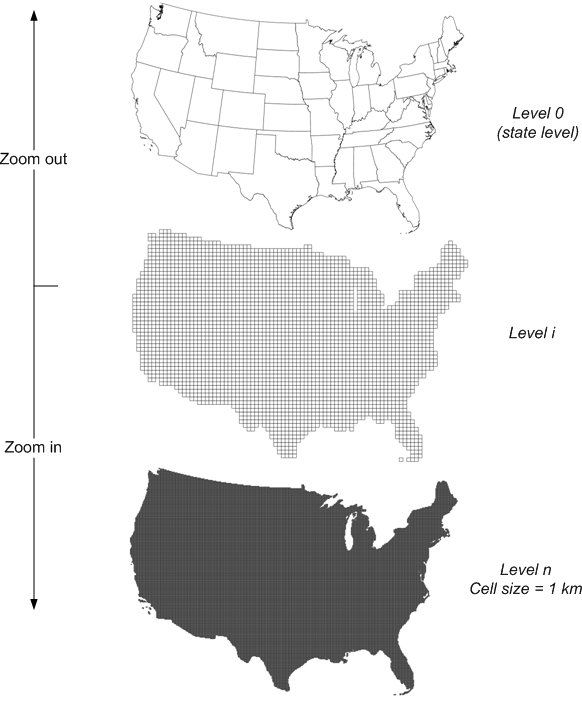
\includegraphics[width=0.6\linewidth]{./figures/multilevel}
\caption{Hierarchical spatial layers for aggregating movements in different level-of-details.}
\label{fig:multilevel}
\end{figure}
\FloatBarrier

\section{Multi-scale Spatiotemporal Twitter User Mobility Patterns}
\subsection{Spatiotemporal Twitter User Mobility Patterns}
The situation of using geo-located tweets as proxies to infer people's movements is complex as users' tweeting behavior can be significantly different from one to another, in particular, the frequency and time-interval between two consecutive tweets.
For example, some people may tweet once a day while others do more; some people may tweet regularly while others do not.  
These tweeting behaviors are expected as such human dynamics are also seen in the mobile phone call data~\cite{gonzalez2008understanding}. 
Many studies have carried out data collection within a certain time period (e.g., a year in our case).
However, as the geo-located tweets were collected in a continuous fashion, it is necessary to examine the sensitivity regarding these behaviors to ensure we are not just capturing a random snapshot from the whole data streams. 

In this study, we have analyzed the cumulative distribution of the frequency Twitter users visiting different locations in the year 2014 (and every month), which uses the methods developed in~\cite{clauset2009power}. 
The frequency is summarized based on the trajectories of individuals extracted from a monthly time span.
Note that different groups of Twitter users may exist in each month. 
It appears that the distribution of the collective Twitter user visitation behaviors in the year 2014 follows a two-tiered power law distributions (shown in Figure~\ref{fig:visitation}.
The majority (the front part) of the distribution follows a truncated power-law distribution $p(x)\sim x^{-\alpha}e^{-\lambda x}$, where $x$ is the number of visited locations and the $\alpha$ value is 1.32.
The tail part (less than 2$\%$ of the whole population) follows a power-law distribution  $p(x)\sim x^{-\alpha}$ with $\alpha$ value is 3.5.
This finding is consistent across all 12 months, with the mean $\alpha$ value as 1.34 $ \pm$  0.05 (standard deviation) and the mean $\lambda$ value as 0.00178 $ \pm$  0.0002 (standard deviation).

The two-tier power law distribution indicates that the collective behaviors of Twitter user visiting different locations can be well approximated with a (truncated) L\'{e}vy Walk model~\cite{ reynolds2012truncated, rhee2011levy}, which has also been identified in many human mobility studies using different mobility data~\cite{zhao2015explaining}.
The similarities among the cumulative distributions suggest that the mobility data collected from geo-located tweets are temporally stable, at least at the monthly interval, which indicates the collected geo-located tweets in one month can potentially reveal similar findings as the ones collected in multiple months.
In addition, the two-tier power law also reveals the diversity in the Twitter user visiting behaviors: (1) a small group Twitter users visited significantly more locations than the others (2) within each group, the probability of Twitter user visiting more locations decreases significantly with a power function.

\begin{figure}[ht]
\centering
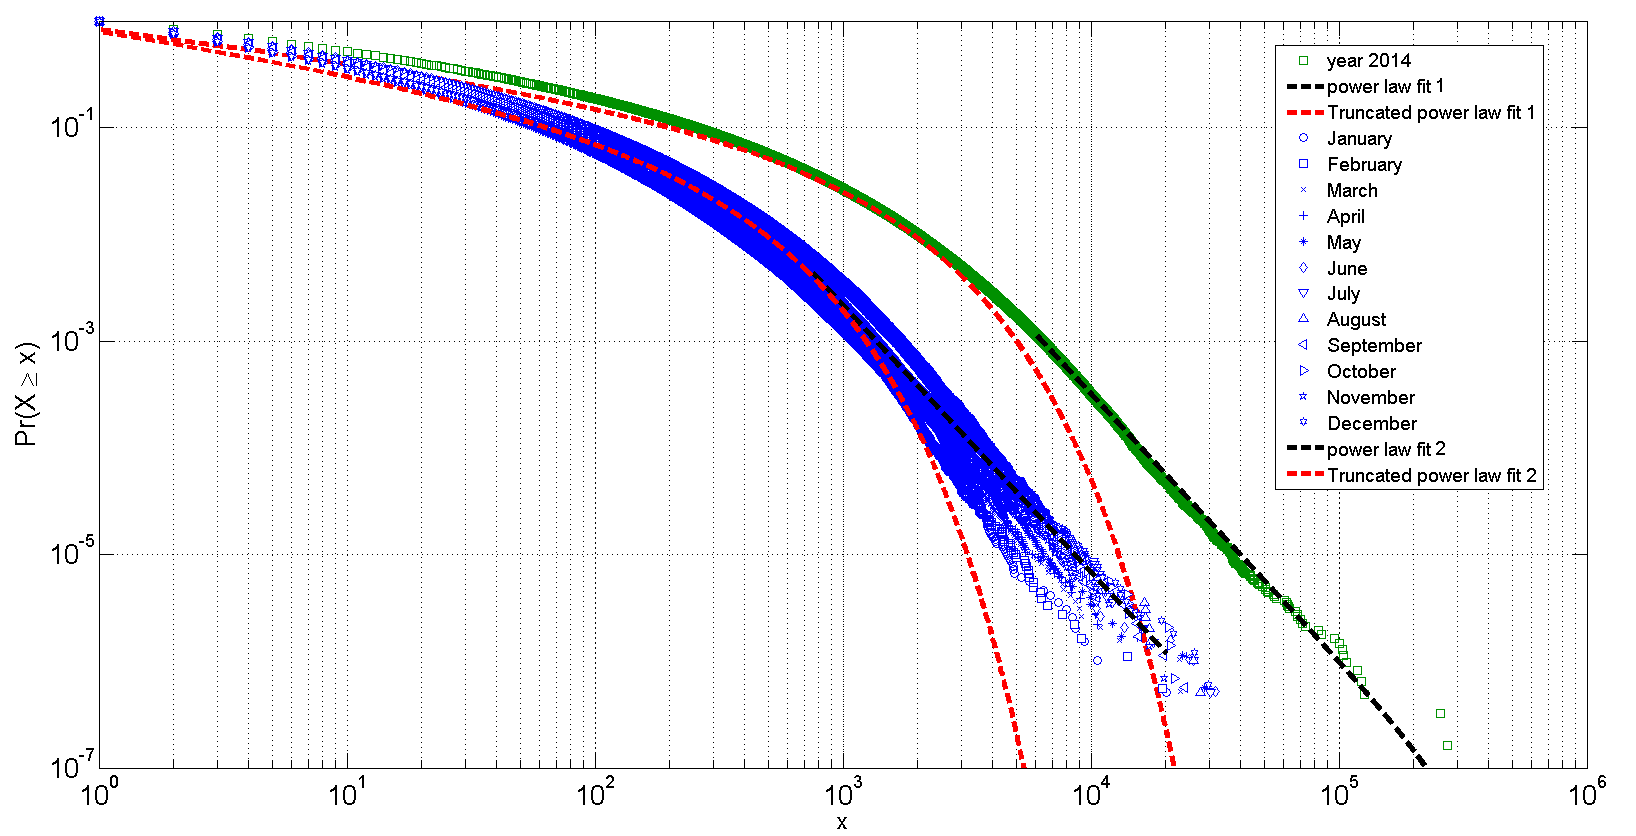
\includegraphics[width=1.0\linewidth]{./figures/visitation}
\caption{Two-tier power law distribution of the collective Twitter user visitation behaviors.}
\label{fig:visitation}
\end{figure}
\FloatBarrier

As it is aforementioned, the measurements of displacements and radius of gyrations of individuals are two popular metrics to quantify the distance decay effects in the collective mobility patterns~\cite{gonzalez2008understanding}.
In this case, we first gathered the displacements from all the collected Twitter users in the continuous United States in the year 2014, where those Twitter users with only one geo-located tweet were filtered out. 
To investigate the mobility patterns of individuals, we also derived the accumulated displacements and the radius of gyrations of each individual Twitter user based on the corresponding space-time trajectories over the one year period.
Note that both displacements and radius of gyrations were calculated by the direct great-circle distance ($d$) between two consecutively recorded locations in a user's trajectory.

To seek mobility patterns from these measurements, we performed statistical analysis regarding the probability distributions of displacements and radius of gyrations, which is also known as the spatial dispersal kernel $P(d)$~\cite{brockmann2006scaling}.
The probability distribution of the user displacements (as well as accumulated displacements) is shown in Figure~\ref{fig:displacement}, whereas the probability distribution of radius of gyrations is shown in Figure~\ref{fig:gyration}. 
In this study, we used the fitting methods developed by~\cite{Jurdak2015}.
The probability distributions of overall displacements, and the accumulated displacements and radius of gyrations of individuals, can all be approximated by a combination of three functions: an exponential function, a stretched-exponential function and a power-law function.

Figure~\ref{fig:displacement}a shows the probability distribution of the overall displacements, which is approximated by $P(d) \sim \lambda_{1} e^{-\lambda_{1}(d - d_{min})}, d_{min}=10~m$ from [10 m, 70 m] (accounting for 2 $\%$ of the population), $ P(d) \sim \beta\lambda_{1}d^{\beta-1}e^{-\lambda^{1}(d^\beta-d_{min}^\beta)}, d_{min}=100~m$ from [100 m, 80 km] (accounting for 93 $\%$ of the population), and $P(d) \sim {d}^{-\alpha}$ [$>$ 80 km] (accounting for 5 $\%$ of the population).
In addition, the displacement in the distance bound from 100 m and 80 km in Figure~\ref{fig:displacement}b can be further approximately by two power-law distributions with a cutting point at 5 km (53$\%$ distances are less than 5 km and 40$\%$ distances between 5 km and 80 km), which indicates two different travel modes, such as inter- or intra-city movements.
Overall, the fitting functions with different distance bounds suggest the existence of multi-scale or multi-modal mobility patterns~\cite{Jurdak2015} of the Twitter users in the continuous United States, for example, the displacements larger than 80 km could be related to inter-state travels and stronger distance decay effects are observed in longer distance travels. 

The probability distribution of radius of gyrations of individuals at the national level (Figure~\ref{fig:gyration}a) is approximated by $P(r_{g}) \sim \lambda_{2} e^{-\lambda_{2}(r_{g} - {r_{g}}_{min})}, {r_{g}}_{min}=10~m$ from [10 m, 50 m], $P(r_{g}) \sim \lambda_{2} e^{-\lambda_{2}(r_{g} - {r_{g}}_{min})}$ from [50 m, 30 km], and $P(r_{g}) \sim {r_{g}}^{-\alpha}$ [$>$ 30 km].
In particular, the radius of gyration between 50 m and 30 km can be further approximately by two power law distributions with a cutting point at 6 km (Figure~\ref{fig:gyration}b), which suggest two main types of spatial coverage of from the collected Twitter users in the continuous United States.
The distribution shows that around $10\%$ the tweet population has a radius of gyration less than 50 meters, which indicates those twitter users mostly tweet at a particular place, such as home or office;  around 60$\%$ of the population has a radius of gyration less than 30 km, which indicates that most of the collected Twitter user movements are ``short'' distances, e.g., within a city locale. Note that the accuracy of these values for defining the distance bound depends on the accuracy of the location information of each geo-located tweet.

\begin{figure}[ht]
\centering
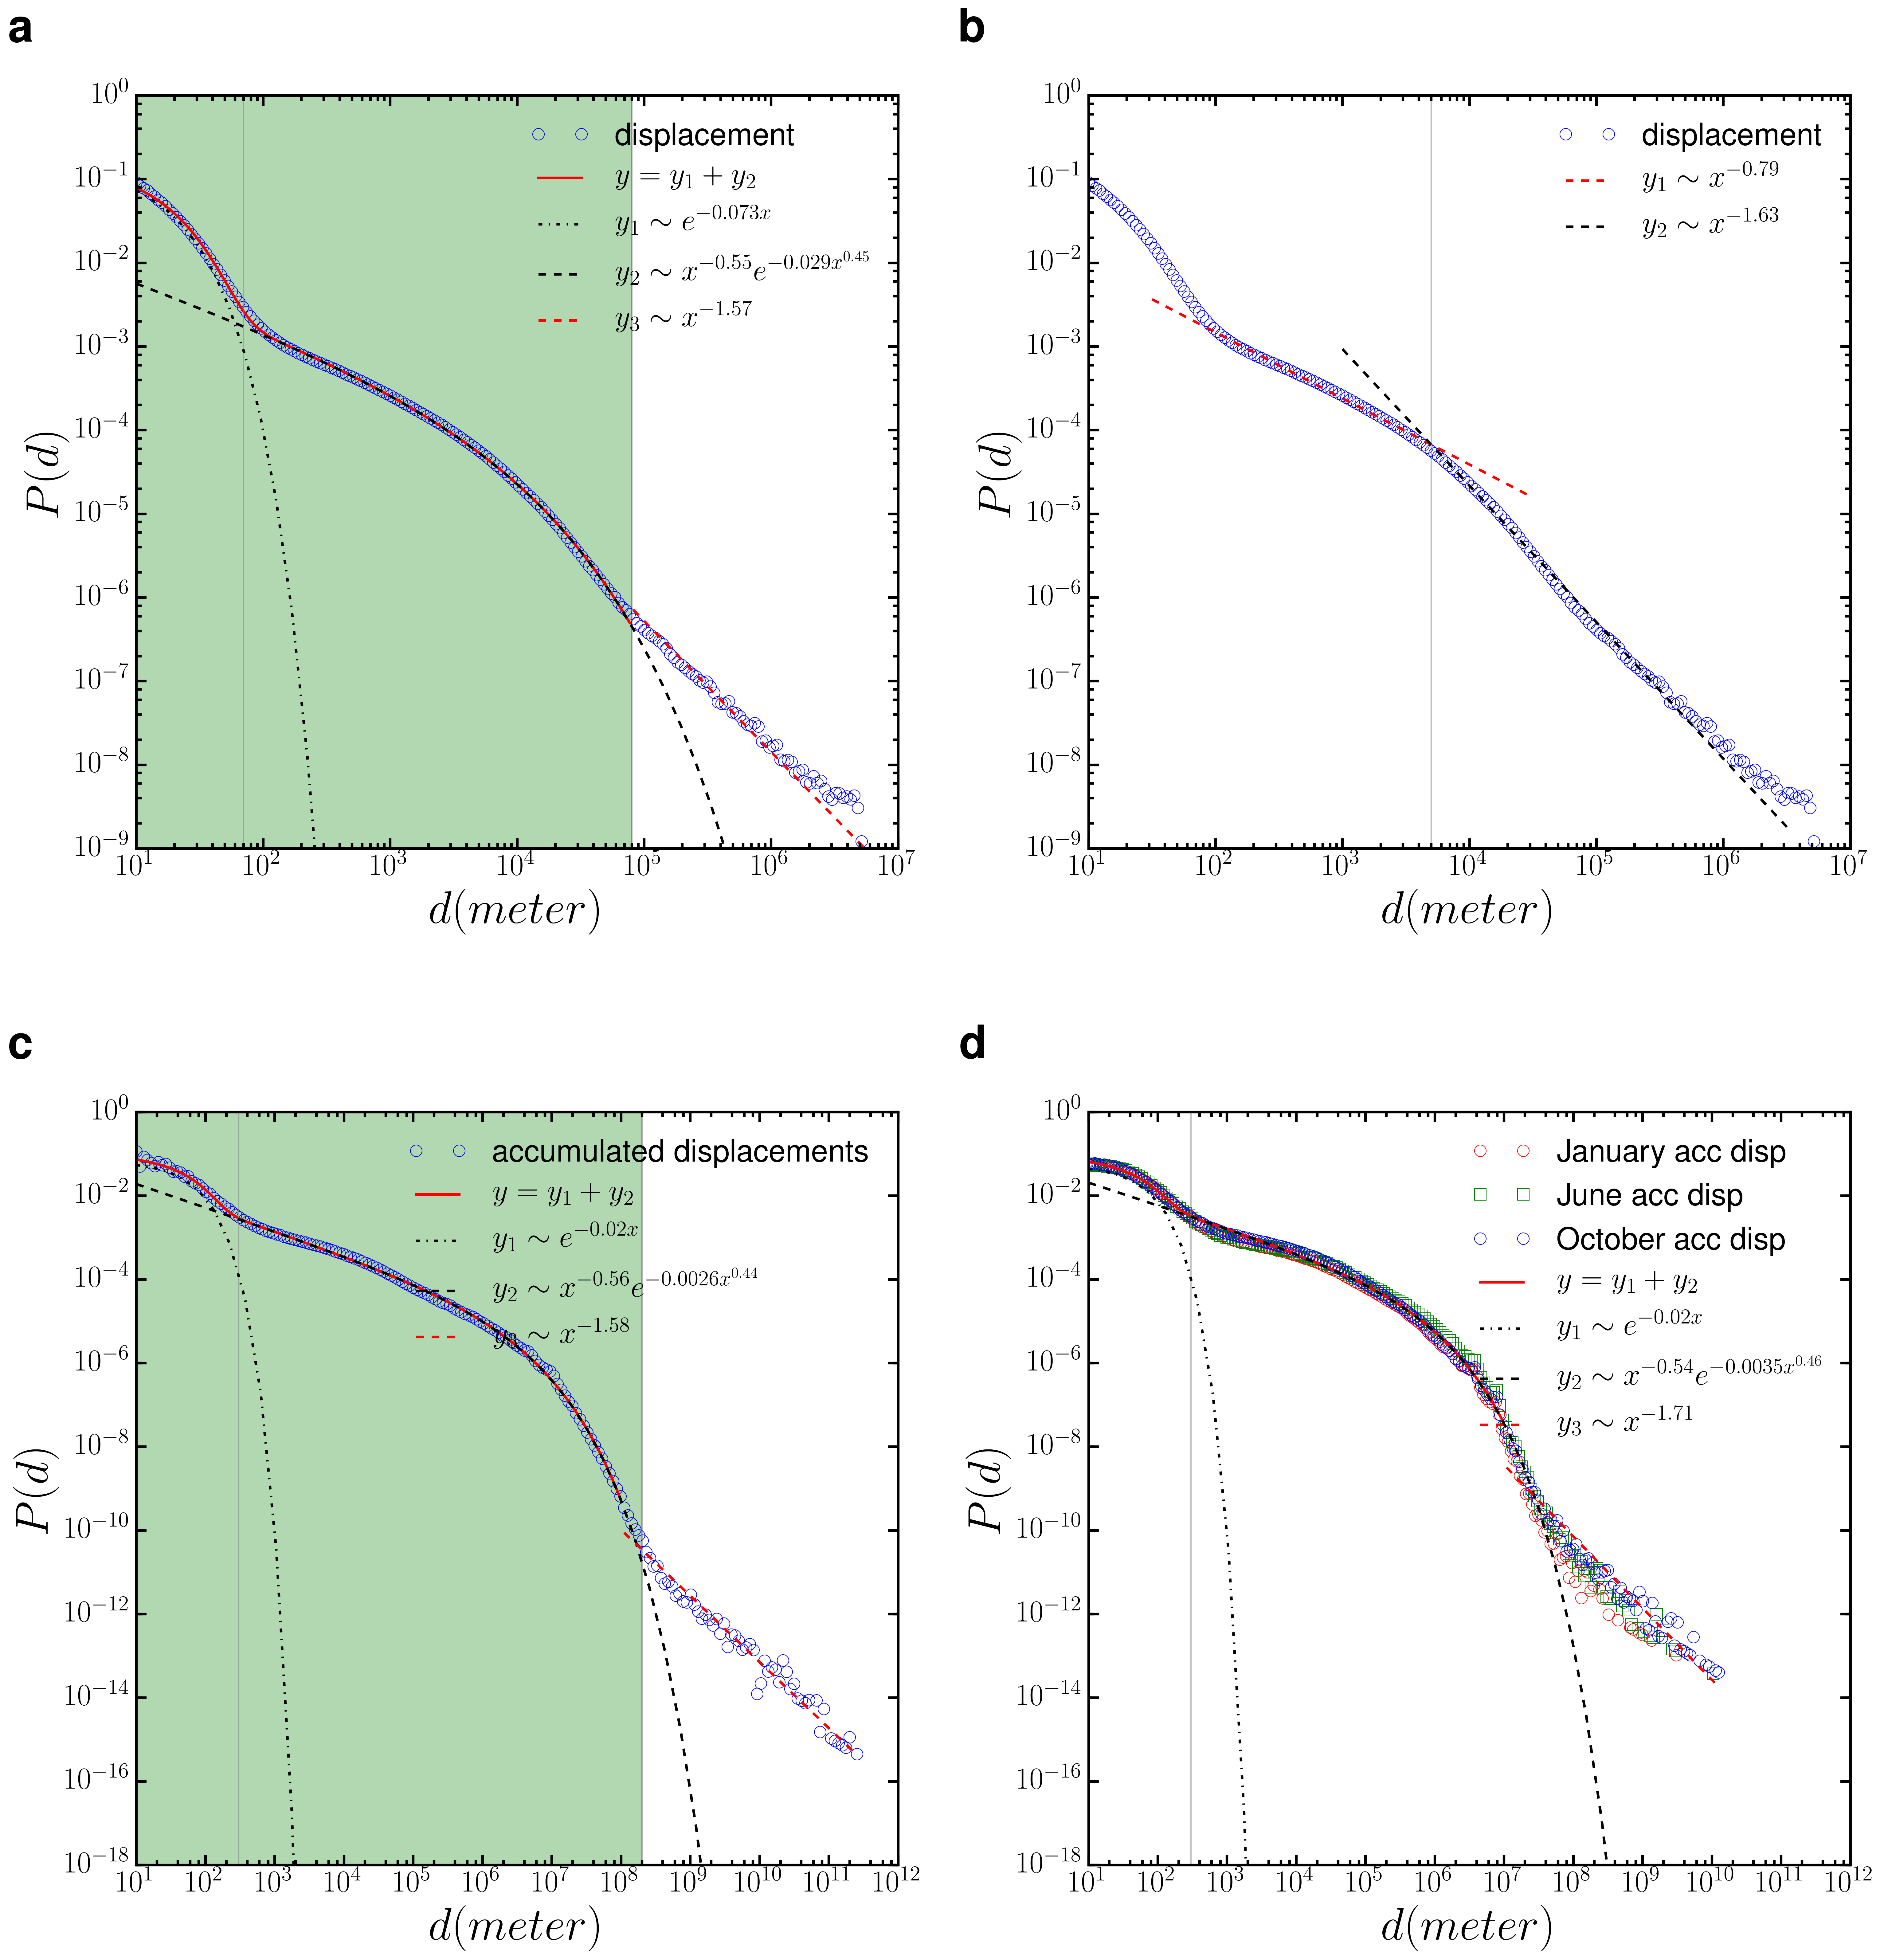
\includegraphics[width=1.0\linewidth]{./figures/displacement}
\caption{({\bf a}) The probability distribution of the collective Twitter user displacements P(d); ({\bf b}) the distance between [100 m, 80 km] is approximated by a double power-law functions; ({\bf c}) The probability distribution of the accumulated displacements of individual Twitter users P(d); ({\bf d}) The probability distribution of the accumulated displacements of individual Twitter users in 3 different months.}

\label{fig:displacement}
\end{figure}
\FloatBarrier

We also measured the distribution of the radius of gyration of Twitter users at different spatial scales, specifically, the state and city level.
In this study, we selected the state Illinois and California for comparisons at the state level (Figure~\ref{fig:gyration}c), whereas we chose Chicago city as an example (Figure~\ref{fig:gyration}d) at the city level.
Interestingly but not surprisingly, the P($r_{g}$) at the state level can also be approximated by a combination of three functions: an exponential function, a stretched-exponential function and a power-law function.
We noticed that distance bound of the radius of gyration at the state level is at 10 km instead of 30 km at the national level.
The distance decay effects in larger spatial coverage [$>$ 30 km] slightly differ, in this case, the P($r_{g}$) decreases faster in smaller size state (i.e., Illinois) than the large size state (i.e., California).
In particular, the P($r_{g}$) over Chicago city can be fitted by similar functions.
However, as it reflects intra-city level mobility patterns, there is no distinct distance range to indicate large spatial coverage.

\begin{figure}[ht]
\centering
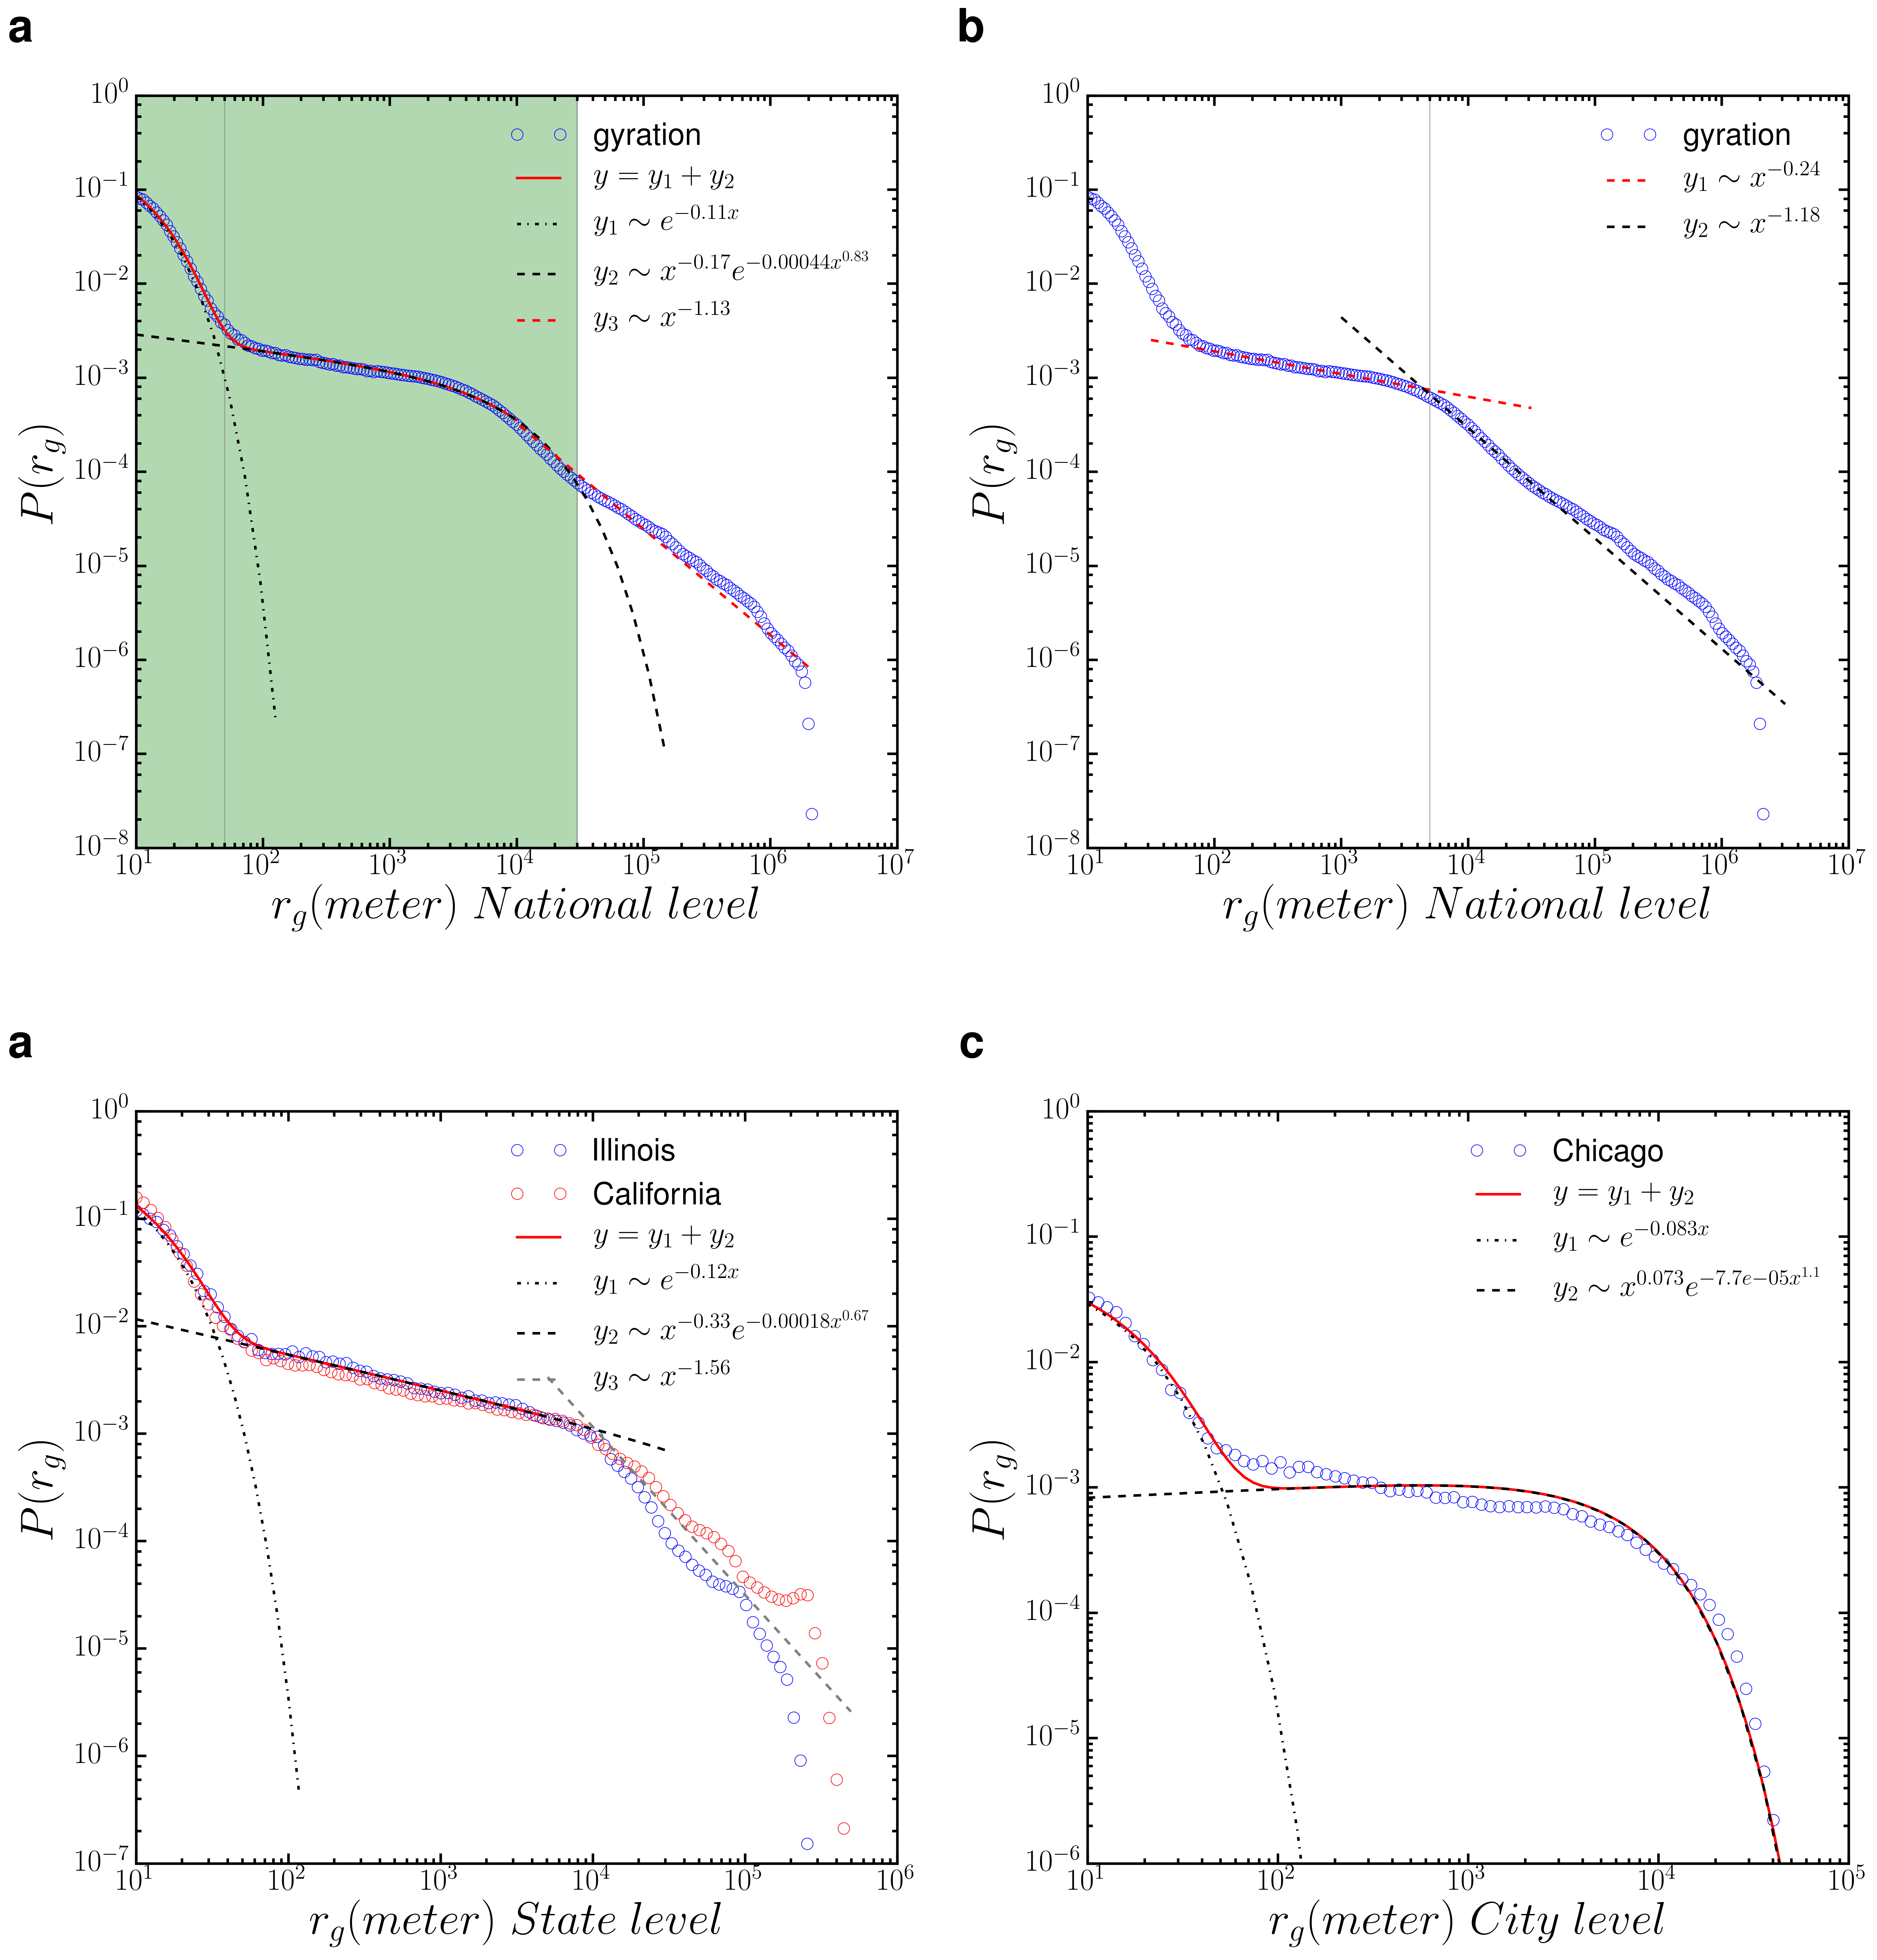
\includegraphics[width=1.0\linewidth]{./figures/gyration2}
\caption{ ({\bf a}) The probability distribution of radius of gyration of individual Twitter users P($r_{g}$) at the national level; ({\bf b}) the distance between [50 m, 30 km] is approximated by a double power-law functions; ({\bf c}) P($r_{g}$) at the state level (Illinois and California); ({\bf d}) P($r_{g}$) for Chicago city.} 
\label{fig:gyration}
\end{figure}
\FloatBarrier

On the other hand, as our framework can aggregate Twitter user trajectories within different temporal ranges, we further analyzed the probability distributions of accumulated displacements took places in January, June, and October (Figure~\ref{fig:displacement}d) and radius of gyrations within 4 quarters in the year 2014 (Figure~\ref{fig:gyration_season}, in order to examine whether there are temporal changes in the mobility patterns.
While the probability distributions of accumulated displacements are almost identical in those selected three months,  we do find changes in the probability distributions of radius of gyrations in different quarters of the year. 
The fluctuations in the tails of the distributions indicate that long distance radius of gyrations (i.e., above 30 km) will experience more seasonal changes in the Twitter user mobility pattern, which means the increase or decrease of long distance movement activities in the corresponding time period. 
However, it is worthy noting that the overall trends in the Twitter user mobility patterns revealed by radius of gyrations are still consistent.

In summary, by comparing these results from different spatial scales and temporal ranges, different distance bounds were identified for describing the spatiotemporal Twitter user mobility patterns.
However, the overall similarity and consistence found, in using a combination of three functions to approximate the probability distribution functions of displacements and radius of gyrations, clearly provide supports for using geo-located tweets as useful proxies for understanding human mobility patterns and conducting reproducible findings at multiple spatial scales and temporal ranges.
 
\begin{figure}[ht]
\centering
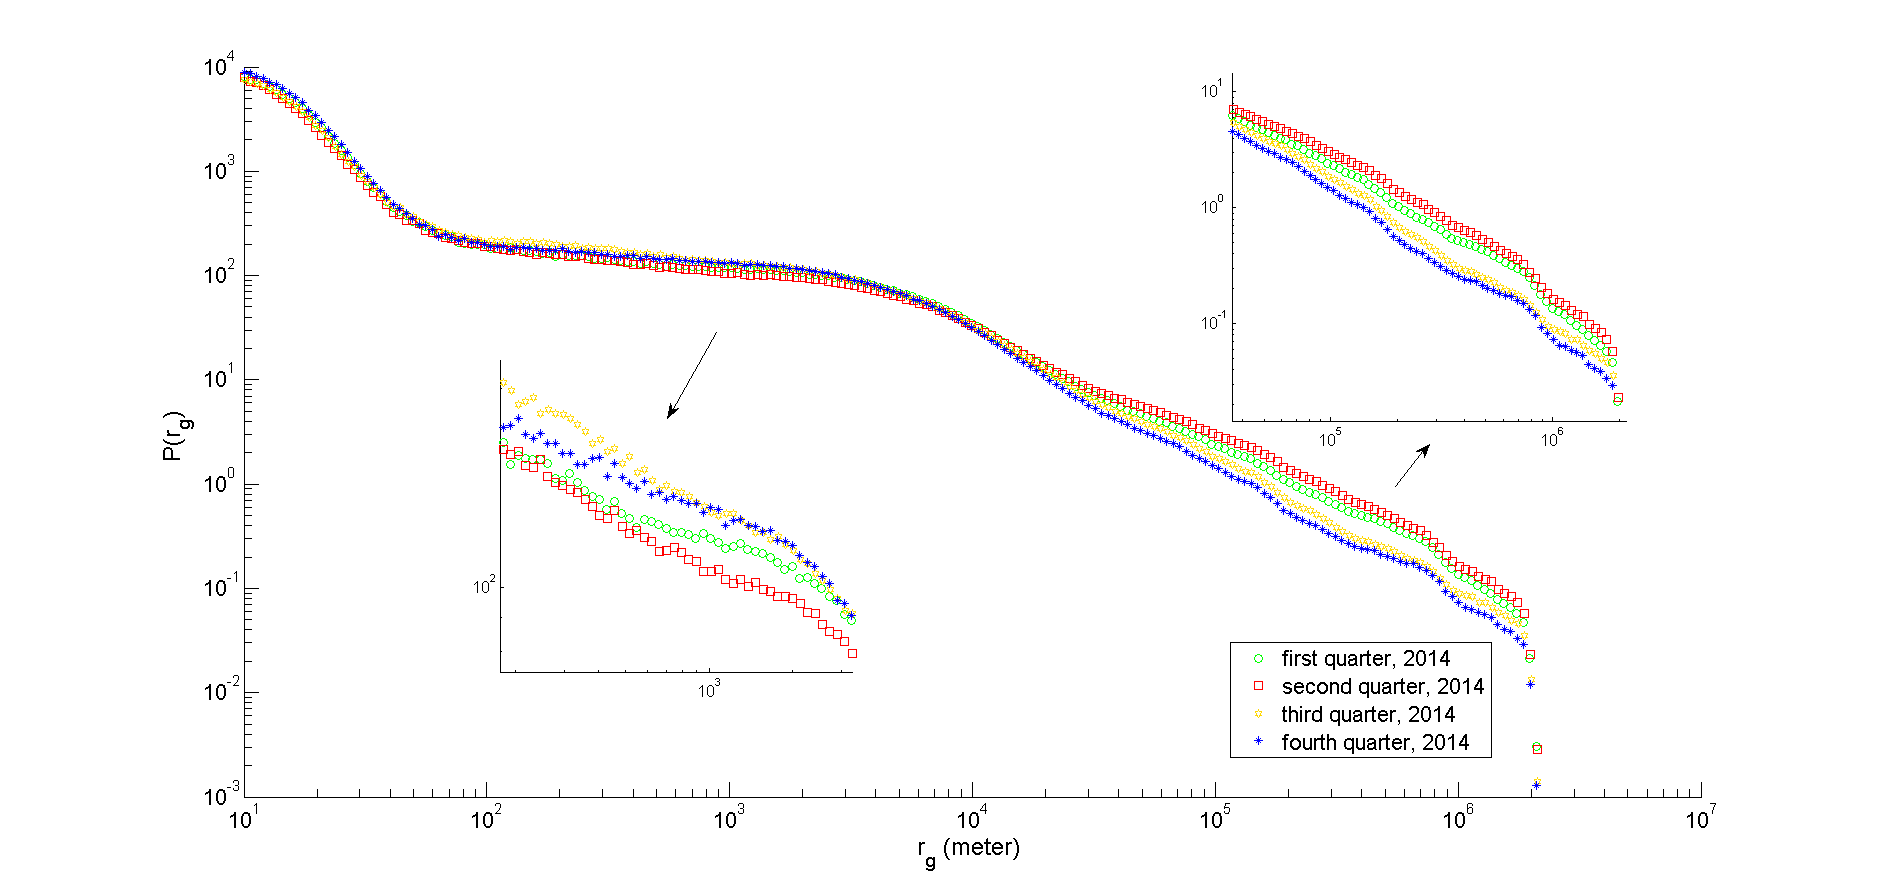
\includegraphics[width=1.0\linewidth]{./figures/gyration_season}
\caption{The probability distribution of radius of gyration of individual Twitter users in different quarters of the year 2014.}
\label{fig:gyration_season}
\end{figure}
\FloatBarrier

The above analysis of Twitter user mobility patterns mainly focuses on the spatiotemporal aspects.
Our framework provides the flexibility to aggregate and extract Twitter user trajectories in a specific spatial scale and re-produce the analysis.
In particular, as it is evident from the above analysis that there are multi-scale or multi-modal Twitter user mobility patterns, this framework can help further look into the mobility pattern regarding how Twitter users move across different spatial scales and temporal ranges, which is measured by the movement flows between these spatial units.
The movement flows are obtained by aggregating the movements that started from and ended in the corresponding spatial units within the giving time frame.
In this case, we demonstrate the inter-state mobility patterns by using the framework to capture the movement flows between the states.
Note that the movement flows can be summarized across all the 10 spatial layers in the framework.
We tested the overall distribution of the movement flows (in the form of weighted in-degree and out-degree of a graph, where each state is treated as a node) among different states in the year 2014.
We found that the probability distribution of Twitter user movement flows of visiting different states follows a log-normal distribution: $p(x)\sim \frac{1}{x}exp[-\frac{(lnx - \mu)^{2}}{2\sigma^{2}}]$, which suggests the flux of Twitter user movements among the states are highly skewed and dominated by a few states (Figure~\ref{fig:state_flow}).
It indicates that the Twitter population is not proportional to account the movement flux between the states, which may provide some insights for other researchers in studying social-economical aspects of the migration dynamics.

\begin{figure}[ht]
\centering
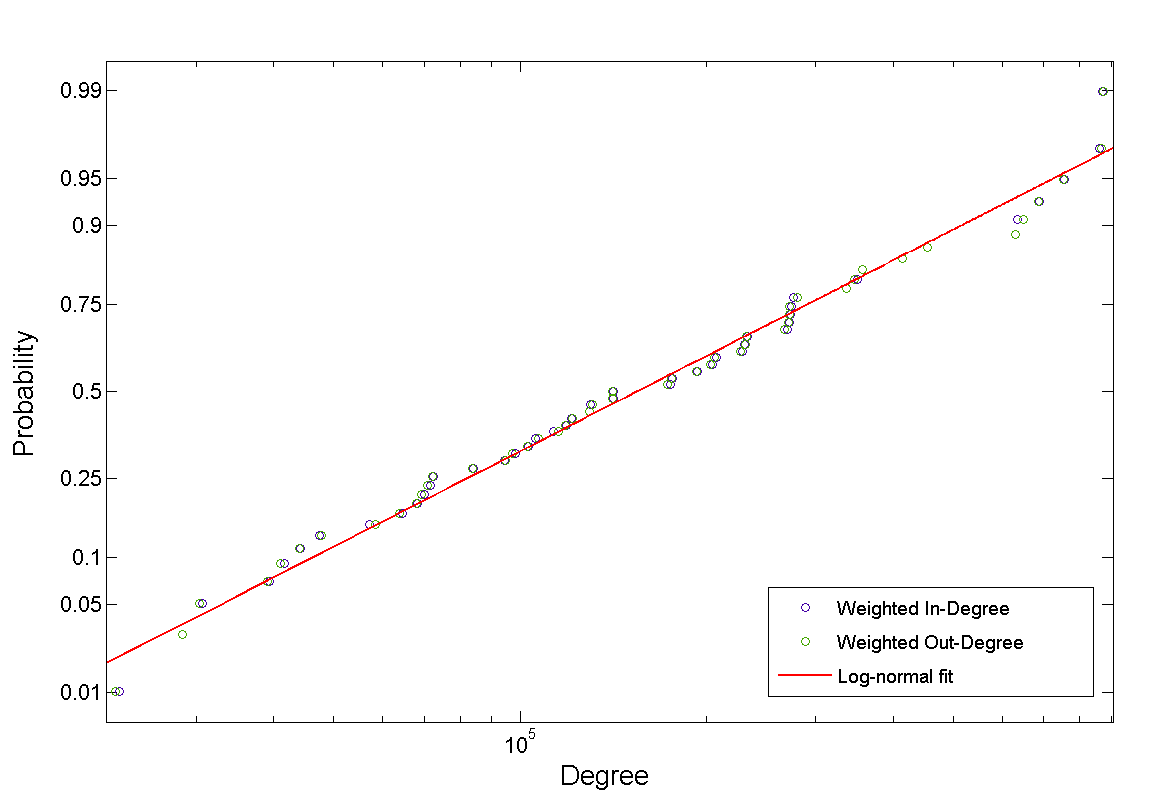
\includegraphics[width=0.8\linewidth]{./figures/degree}
\caption{The distribution of Twitter user movement flows among different states in the year 2014 measured in weighted in- and out-degrees.}
\label{fig:state_flow}
\end{figure}
\FloatBarrier

\subsection{The Interactive 3D Virtual Globe Web Mapping Interface}
In addition to providing supports for understanding Twitter user mobility patterns with statistical analysis, the framework integrates a 3D virtual globe interface to enable users to perform exploratory geo-visual analytics of the multi-level spatiotemporal Twitter user movements (http://sandbox.cigi.illinois.edu/home). 
The 3D virtual globe is developed and extended from the Cesium library (http://cesiumjs.org), which is an open-source WebGL virtual globe and map engine.
We customized the map engine to adapt different spatial scales, which correspond to the hierarchical spatial layers, for aggregating movements in different levels-of-detail.
The map interface interprets user's interactions, such as area-of-interest, time window, and zoom levels, etc. as parameters and send to the dedicated visualization servlet on the CyberGIS Gateway, which is the leading online cyberGIS environment for a large number of users to perform computing- and data-intensive, and collaborative geospatial problem-solving enabled by advanced cyberinfrastructure~\cite{liu2014cybergis}.

An overview of the 3D web mapping interface is shown in Figure~\ref{fig:Web_Interface}.
The mapping interface visualizes the corresponding movement flows on the virtual globe, where the number of movement flows are divided by 20 percentiles and categorized by the colors shown in the legend.
In terms of performing exploratory visual-analytics of Twitter user movement patterns, users can specify the time window to enable the query. 
When the results are shown, users can hover the mouse over each individual lines on the map to see the value of movement flows for both in and out directions (highlighted in color green).
If the selected criteria keep unchanged, whenever the user zooms in/out, tilt or rotate the globe, the 3D virtual globe mapping interface will automatically provide the corresponding level-of-details on the fly.
For example, Figure~\ref{fig:chicago} and Figure~\ref{fig:Chicago_airport} demonstrated the movement flows in different level-of-details around the Chicago city, and between O'Hare International Airport and the city center of Chicago city, where top 20$\%$ movement flows were shown.
The 3D mapping interface facilitates uses to query multi-scale Twitter user movements with a geographical context and in an interactive fashion.
For example, users can perform comparative studies of Twitter user movements in different cities by simply rotating the globe. 
More importantly, this mapping interface can be easily customized and extended to accommodate future geo-located Twitter data collection with larger spatial coverages.
The source code of the visual-analytics framework in this paper is available upon request.

\begin{figure}[ht]
\centering
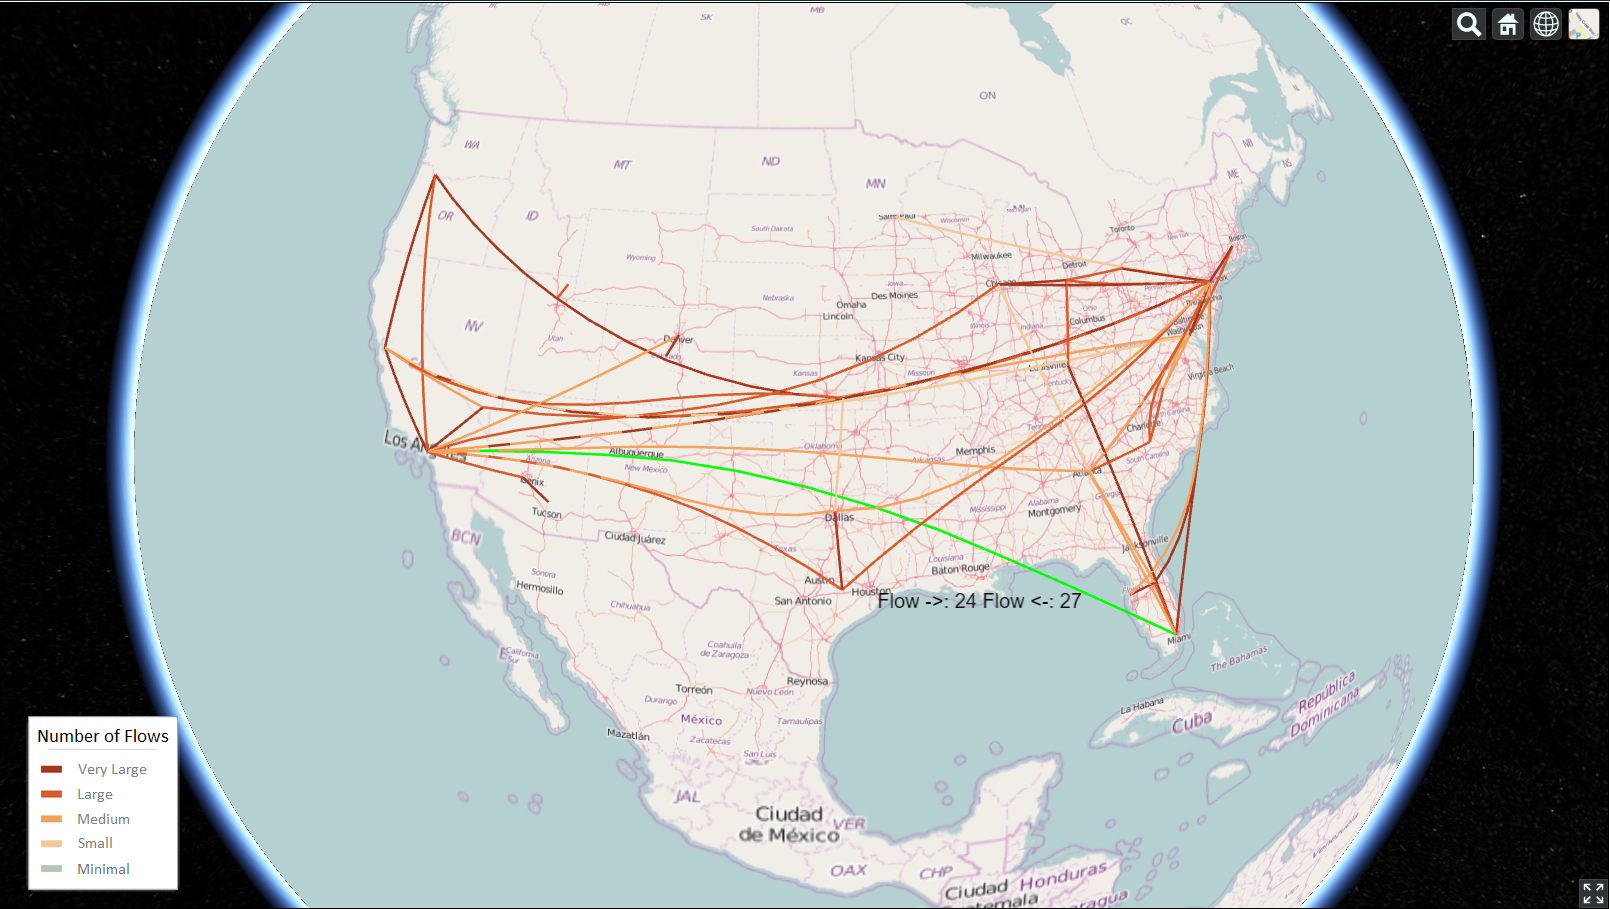
\includegraphics[width=0.8\linewidth]{./figures/all}
\caption{An overview of the 3D interactive web mapping interface.}
\label{fig:Web_Interface}
\end{figure}
\FloatBarrier

\begin{figure}[ht]
\centering
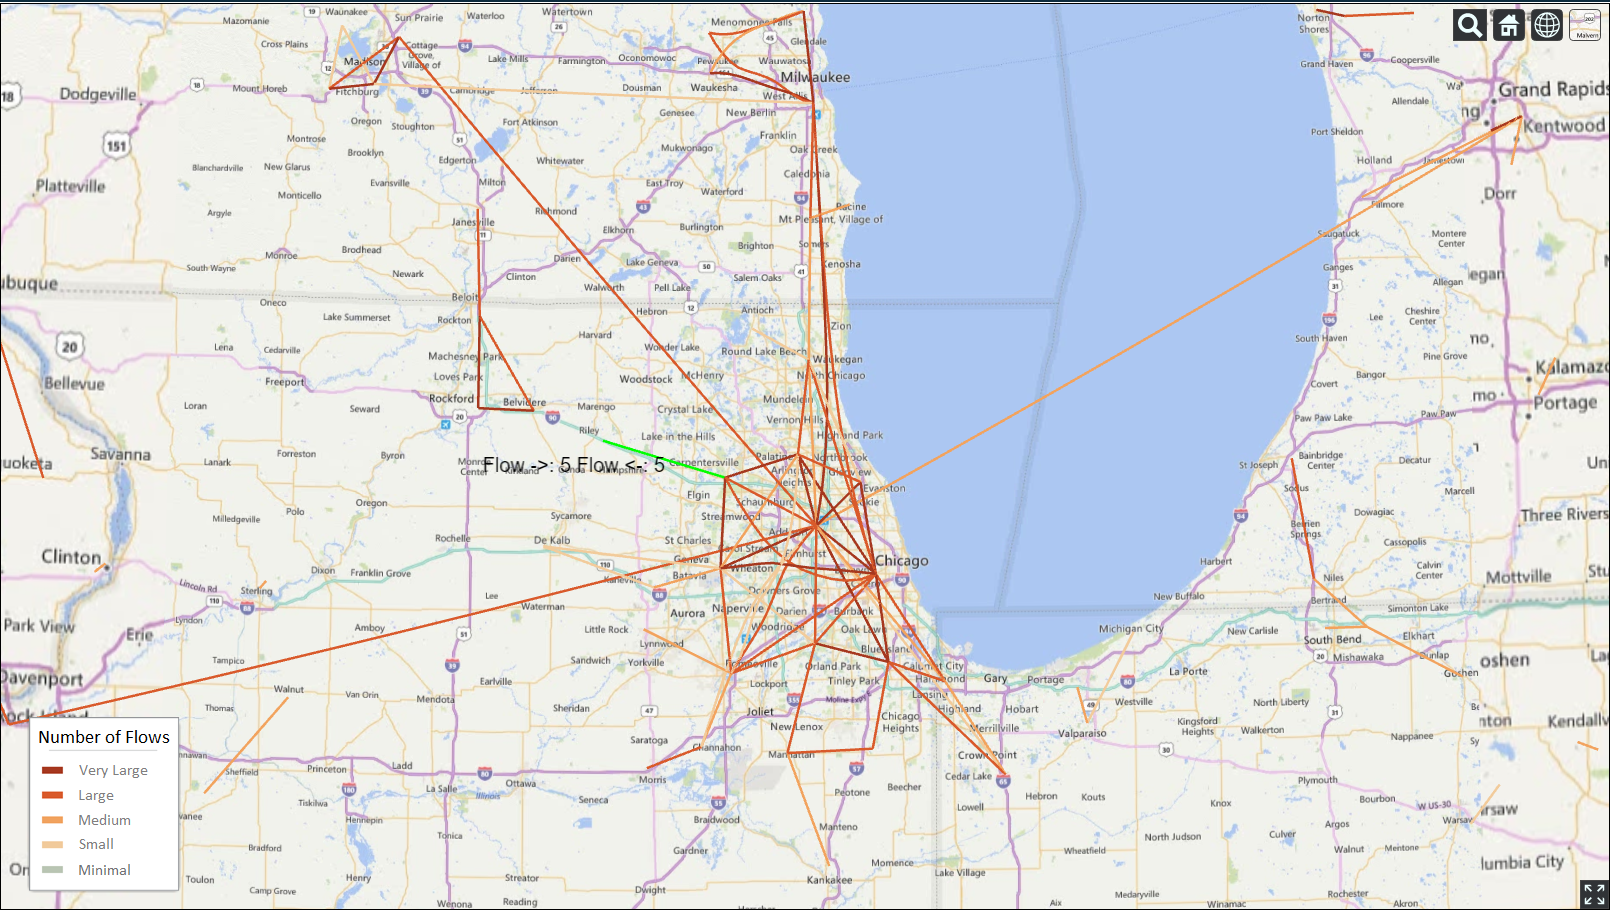
\includegraphics[width=0.8\linewidth]{./figures/Chicago}
\caption{The top 20$\%$ movement flows around Chicago city.}
\label{fig:chicago}
\end{figure}
\FloatBarrier

\begin{figure}[ht]
\centering
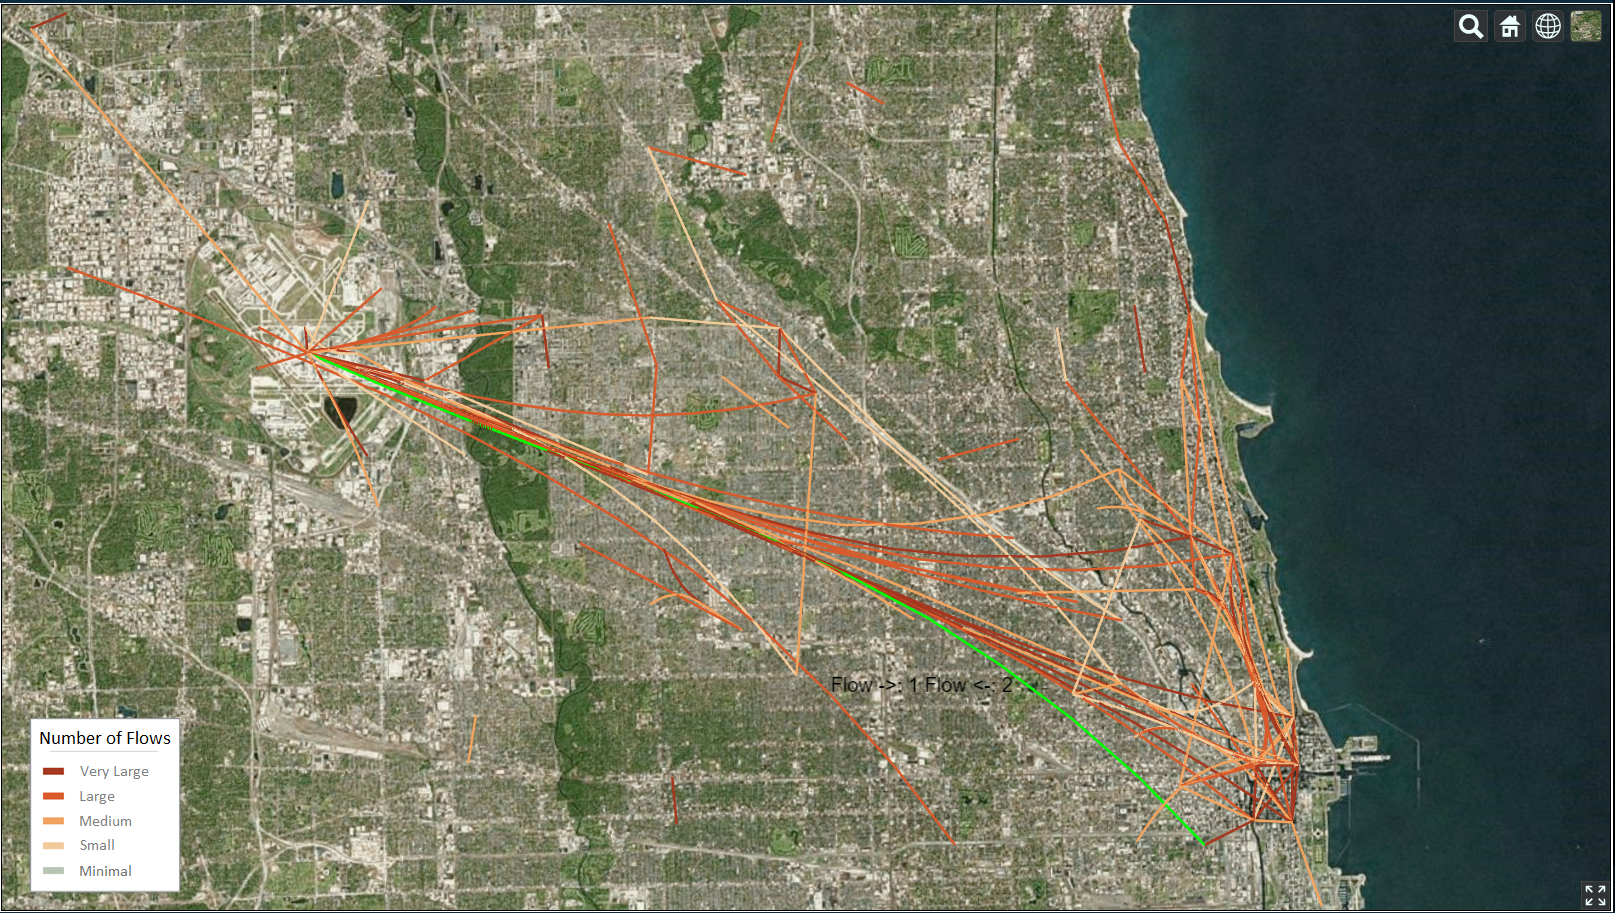
\includegraphics[width=0.8\linewidth]{./figures/Chicago_airport}
\caption{The top 20$\%$ movement flows between O'Hare International Airport and the city center of Chicago city.}
\label{fig:Chicago_airport}
\end{figure}
\FloatBarrier

\section{Conclusions}
In this study, we have used large volume of geo-located tweets to study Twitter user mobility patterns across multi-level spatial scales and temporal ranges in the continuous United States during the year 2014. 
To address the data-intensive challenges, we have developed a scalable visual-analytics framework tailored to accommodate large volume of geo-located tweets for studying multi-scale spatiotemporal Twitter user mobility patterns.
This framework is implemented on high-performance distributed computing environment using Apache Hadoop.
It provides efficiency in filtering large volume of geo-located tweets, modeling and extracting Twitter user movements, generating space-time user trajectories, and summarizing multi-level spatiotemporal user mobility patterns. For example, we have included an experiment for illustrating the processing time regarding generating Twitter user trajectories across different time span in the supplement material.

With this framework, we have found some interesting Twitter user mobility patterns, both statistically and visually.
We studied the collective Twitter user visiting behavior regarding the frequency of Twitter users visiting different locations, which was fitted by a two-tier power-law distribution function.
The two-tier power law distribution indicates that the collective behaviors of Twitter user visiting different locations can be well approximated with a (truncated) L\'{e}vy Walk model, which has also been identified in many human mobility studies using different mobility data.
The similarities among the cumulative distributions suggest that the mobility data collected from geo-located tweets are temporally stable, at least at the monthly interval, which provides supports that we are not just capturing a random snapshot of the whole data stream. 

We studied the distance decay effects in the collective Twitter user movements measured by the probability distributions of the displacements and radius of gyrations of individuals. 
These distributions can all be approximated by a combination of three functions: an exponential function, a stretched-exponential function and a power-law function. In particular, distance bounds between different fitting functions in displacement distribution reveals the existence of multi-scale or multi-modal mobility patterns of the Twitter users, whereas the distribution of radius of gyration reveals different groups of Twitter users with different types of spatial coverages at multiple spatial scales.   
We further studied these mobility patterns in different temporal ranges to investigate the temporal changes in the mobility patterns. 
We found that the accumulated displacements are almost identical in different months, while the long distance radius of gyration (i.e., above 30 km) will experience more seasonal changes in the Twitter user mobility pattern.

Finally, it is worth noting that at the current stage the geo-located Twitter data is not able to generalize to the entire population.
As the demographic information of the Twitter users cannot be easily identified, the results derived in this study may not reflect a complete real-world image of human movements, which should be carefully considered in future studies.
Nevertheless, the Twitter user movements provide clear supports to reveal the distance decay effects in human mobility research, which is observed in multiple spatial and temporal scales.
Due to the large sample size, it is difficult to generalize the mobility pattern found at national level to entire population, city-level mobility pattern may provide better insights for investigating mobility dynamics. For example, the results of radius of gyration in Chicago exhibit similar pattern found in larger spatial scale, and with inputs of other mobility dataset that are often available at city-level, such as taxi trip records and mobile phone call data, there is a potential to synthesize these different sources of information and therefore provide a more complete image for understanding human mobility patterns.
On the other hand, as we have discussed in this paper that geo-located Twitter data show the advantages regarding the easy data accessibility, the large spatial coverage and massive sample size, our approach took advantage of such data source to understand the mobility patterns across multiple spatial scales and temporal ranges.
Also, our approach can be applied to the setting of other countries, which can be used to carry out comparative studies regarding spatiotemporal Twitter user mobility patterns. 


%%%%%%%%%%%%%%%%%%%%%%%%%%%%%%%%%%%%%%%%%%
%% optional
%\supplementary{The following are available online at www.mdpi.com/link, Figure S1: title, Table S1: title, Video S1: title.}

%%%%%%%%%%%%%%%%%%%%%%%%%%%%%%%%%%%%%%%%%%
\acknowledgments{
The authors would like to thank the four anonymous reviewers of IJGI for their constructive comments that better shaped the paper.
Junjun Yin would like to thank the funding support from the U.S. National Science Foundation under grant numbers: ACI-1047916, BCS-0846655, and IIS-1354329.
Zhenhong Du would like to thank the funding support from the Fundamental Research Funds for the Central Universities under grant number:2016XZZX004-02.
The work also used the ROGER supercomputer, which is supported by NSF under grant number: 1429699.}

%%%%%%%%%%%%%%%%%%%%%%%%%%%%%%%%%%%%%%%%%%
\authorcontributions{Junjun Yin conceived and designed the experiments; Junjun Yin and Zhenhong Du analyzed the results; Junjun Yin and Zhenhong Du wrote the paper.}

%%%%%%%%%%%%%%%%%%%%%%%%%%%%%%%%%%%%%%%%%%
\conflictofinterests{The authors declare no conflict of interest. The founding sponsors had no role in the design of the study; in the collection, analyses, or interpretation of data; in the writing of the manuscript, and in the decision to publish the results.} 

%%%%%%%%%%%%%%%%%%%%%%%%%%%%%%%%%%%%%%%%%%
\renewcommand\bibname{References}
\begin{thebibliography}{-------}
\providecommand{\natexlab}[1]{#1}
\providecommand{\natexlab}[1]{#1}

\bibitem[Zheng \em{et~al.}(2008)Zheng, Li, Chen, Xie, and
  Ma]{zheng2008understanding}
Zheng, Y.; Li, Q.; Chen, Y.; Xie, X.; Ma, W.Y.
\newblock Understanding mobility based on GPS data.
\newblock  Proceedings of the 10th international conference on Ubiquitous
  computing. ACM,  2008, pp. 312--321.

\bibitem[Jiang \em{et~al.}(2009)Jiang, Yin, and Zhao]{jiang2009characterizing}
Jiang, B.; Yin, J.; Zhao, S.
\newblock Characterizing the human mobility pattern in a large street network.
\newblock {\em Physical Review E} {\bf 2009}, {\em 80},~021136.

\bibitem[Belik \em{et~al.}(2011)Belik, Geisel, and Brockmann]{belik2011natural}
Belik, V.; Geisel, T.; Brockmann, D.
\newblock Natural human mobility patterns and spatial spread of infectious
  diseases.
\newblock {\em Physical Review X} {\bf 2011}, {\em 1},~011001.

\bibitem[Greenwood(1985)]{greenwood1985human}
Greenwood, M.J.
\newblock Human migration: Theory, models, and empirical studies.
\newblock {\em Journal of regional Science} {\bf 1985}, {\em 25},~521--544.

\bibitem[Brockmann \em{et~al.}(2006)Brockmann, Hufnagel, and
  Geisel]{brockmann2006scaling}
Brockmann, D.; Hufnagel, L.; Geisel, T.
\newblock The scaling laws of human travel.
\newblock {\em Nature} {\bf 2006}, {\em 439},~462--465.

\bibitem[Gonzalez \em{et~al.}(2008)Gonzalez, Hidalgo, and
  Barabasi]{gonzalez2008understanding}
Gonzalez, M.C.; Hidalgo, C.A.; Barabasi, A.L.
\newblock Understanding individual human mobility patterns.
\newblock {\em Nature} {\bf 2008}, {\em 453},~779--782.

\bibitem[Jurdak \em{et~al.}(2015)Jurdak, Zhao, Liu, AbouJaoude, Cameron, and
  Newth]{Jurdak2015}
Jurdak, R.; Zhao, K.; Liu, J.; AbouJaoude, M.; Cameron, M.; Newth, D.
\newblock Understanding Human Mobility from Twitter.
\newblock {\em PLoS ONE} {\bf 2015}, {\em 10},~e0131469.

\bibitem[Rhee \em{et~al.}(2011)Rhee, Shin, Hong, Lee, Kim, and
  Chong]{rhee2011levy}
Rhee, I.; Shin, M.; Hong, S.; Lee, K.; Kim, S.J.; Chong, S.
\newblock On the levy-walk nature of human mobility.
\newblock {\em IEEE/ACM transactions on networking (TON)} {\bf 2011}, {\em
  19},~630--643.

\bibitem[Sevtsuk and Ratti(2010)]{sevtsuk2010does}
Sevtsuk, A.; Ratti, C.
\newblock Does urban mobility have a daily routine? Learning from the aggregate
  data of mobile networks.
\newblock {\em Journal of Urban Technology} {\bf 2010}, {\em 17},~41--60.

\bibitem[Kung \em{et~al.}(2014)Kung, Greco, Sobolevsky, and
  Ratti]{kung2014exploring}
Kung, K.S.; Greco, K.; Sobolevsky, S.; Ratti, C.
\newblock Exploring universal patterns in human home-work commuting from mobile
  phone data.
\newblock {\em PloS one} {\bf 2014}, {\em 9},~e96180.

\bibitem[Thatcher(2014)]{thatcher2014living}
Thatcher, J.
\newblock Living on fumes: Digital footprints, data fumes, and the limitations
  of spatial big data.
\newblock {\em International Journal of Communication} {\bf 2014}, {\em
  8},~1765--1783.

\bibitem[Hawelka \em{et~al.}(2014)Hawelka, Sitko, Beinat, Sobolevsky,
  Kazakopoulos, and Ratti]{hawelka2014geo}
Hawelka, B.; Sitko, I.; Beinat, E.; Sobolevsky, S.; Kazakopoulos, P.; Ratti, C.
\newblock Geo-located Twitter as proxy for global mobility patterns.
\newblock {\em Cartography and Geographic Information Science} {\bf 2014}, {\em
  41},~260--271.

\bibitem[Giannotti and Pedreschi(2008)]{giannotti2008mobility}
Giannotti, F.; Pedreschi, D.
\newblock {\em Mobility, data mining and privacy: Geographic knowledge
  discovery}; Springer Science \& Business Media,  2008.

\bibitem[Crampton(2014)]{crampton2014collect}
Crampton, J.W.
\newblock Collect it all: national security, Big Data and governance.
\newblock {\em GeoJournal} {\bf 2014}, pp. 1--13.

\bibitem[Wu \em{et~al.}(2014)Wu, Zhi, Sui, and Liu]{wu2014intra}
Wu, L.; Zhi, Y.; Sui, Z.; Liu, Y.
\newblock Intra-urban human mobility and activity transition: Evidence from
  social media check-in data.
\newblock {\em PloS one} {\bf 2014}, {\em 9},~e97010.

\bibitem[Hasan \em{et~al.}(2013)Hasan, Zhan, and
  Ukkusuri]{hasan2013understanding}
Hasan, S.; Zhan, X.; Ukkusuri, S.V.
\newblock Understanding urban human activity and mobility patterns using
  large-scale location-based data from online social media.
\newblock  Proceedings of the 2nd ACM SIGKDD international workshop on urban
  computing. ACM,  2013, p.~6.

\bibitem[Cho \em{et~al.}(2011)Cho, Myers, and Leskovec]{cho2011friendship}
Cho, E.; Myers, S.A.; Leskovec, J.
\newblock Friendship and mobility: user movement in location-based social
  networks.
\newblock  Proceedings of the 17th ACM SIGKDD international conference on
  Knowledge discovery and data mining. ACM,  2011, pp. 1082--1090.

\bibitem[Noulas \em{et~al.}(2012)Noulas, Scellato, Lambiotte, Pontil, and
  Mascolo]{noulas2012tale}
Noulas, A.; Scellato, S.; Lambiotte, R.; Pontil, M.; Mascolo, C.
\newblock A tale of many cities: universal patterns in human urban mobility.
\newblock {\em PloS one} {\bf 2012}, {\em 7},~e37027.

\bibitem[Balcan \em{et~al.}(2009)Balcan, Colizza, Gon{\c{c}}alves, Hu, Ramasco,
  and Vespignani]{balcan2009multiscale}
Balcan, D.; Colizza, V.; Gon{\c{c}}alves, B.; Hu, H.; Ramasco, J.J.;
  Vespignani, A.
\newblock Multiscale mobility networks and the spatial spreading of infectious
  diseases.
\newblock {\em Proceedings of the National Academy of Sciences} {\bf 2009},
  {\em 106},~21484--21489.

\bibitem[Tamerius \em{et~al.}(2011)Tamerius, Nelson, Zhou, Viboud, Miller, and
  Alonso]{tamerius2011global}
Tamerius, J.; Nelson, M.I.; Zhou, S.Z.; Viboud, C.; Miller, M.A.; Alonso, W.J.
\newblock Global influenza seasonality: reconciling patterns across temperate
  and tropical regions.
\newblock {\em Environmental health perspectives} {\bf 2011}, {\em 119},~439.

\bibitem[Tsou(2015)]{tsou2015}
Tsou, M.H.
\newblock Research challenges and opportunities in mapping social media and Big
  Data.
\newblock {\em Cartography and Geographic Information Science} {\bf 2015}, {\em
  42},~70--74.

\bibitem[Zheng \em{et~al.}(2010)Zheng, Xie, and Ma]{zheng2010geolife}
Zheng, Y.; Xie, X.; Ma, W.Y.
\newblock GeoLife: A Collaborative Social Networking Service among User,
  Location and Trajectory. {\bf 2010}.

\bibitem[Becker \em{et~al.}(2013)Becker, C{\'a}ceres, Hanson, Isaacman, Loh,
  Martonosi, Rowland, Urbanek, Varshavsky, and Volinsky]{becker2013human}
Becker, R.; C{\'a}ceres, R.; Hanson, K.; Isaacman, S.; Loh, J.M.; Martonosi,
  M.; Rowland, J.; Urbanek, S.; Varshavsky, A.; Volinsky, C.
\newblock Human mobility characterization from cellular network data.
\newblock {\em Communications of the ACM} {\bf 2013}, {\em 56},~74--82.

\bibitem[Sobolevsky \em{et~al.}(2013)Sobolevsky, Szell, Campari, Couronn{\'e},
  Smoreda, and Ratti]{sobolevsky2013delineating}
Sobolevsky, S.; Szell, M.; Campari, R.; Couronn{\'e}, T.; Smoreda, Z.; Ratti,
  C.
\newblock Delineating geographical regions with networks of human interactions
  in an extensive set of countries.
\newblock {\em PLoS One} {\bf 2013}, {\em 8},~e81707.

\bibitem[Twitter(2016)]{twitterAPI}
Twitter.
\newblock Twitter streaming API.
\newblock {\em available from: https://dev.twitter.com/streaming/overview} {\bf
  2016}.

\bibitem[Cranshaw \em{et~al.}(2012)Cranshaw, Schwartz, Hong, and
  Sadeh]{cranshaw2012livehoods}
Cranshaw, J.; Schwartz, R.; Hong, J.I.; Sadeh, N.M.
\newblock The Livehoods Project: Utilizing Social Media to Understand the
  Dynamics of a City.
\newblock  ICWSM,  2012.

\bibitem[Mitchell \em{et~al.}(2013)Mitchell, Frank, Harris, Dodds, and
  Danforth]{mitchell2013geography}
Mitchell, L.; Frank, M.R.; Harris, K.D.; Dodds, P.S.; Danforth, C.M.
\newblock The geography of happiness: Connecting twitter sentiment and
  expression, demographics, and objective characteristics of place {\bf 2013}.

\bibitem[Longley \em{et~al.}(2015)Longley, Adnan, Lansley,
  et~al.]{longley2015geotemporal}
Longley, P.A.; Adnan, M.; Lansley, G.; others.
\newblock The geotemporal demographics of Twitter usage.
\newblock {\em Environment and Planning A} {\bf 2015}, {\em 47},~465--484.

\bibitem[H{\"a}gerstrand \em{et~al.}(1985)H{\"a}gerstrand
  et~al.]{hagerstrand1985time}
H{\"a}gerstrand, T.; others.
\newblock Time-geography: focus on the corporeality of man, society, and
  environment.
\newblock {\em The science and praxis of complexity} {\bf 1985}, pp. 193--216.

\bibitem[Kwan and Lee(2004)]{kwan2004geovisualization}
Kwan, M.P.; Lee, J.
\newblock Geovisualization of human activity patterns using 3D GIS: a
  time-geographic approach.
\newblock {\em Spatially integrated social science} {\bf 2004}, {\em 27}.

\bibitem[Andrienko and Andrienko(2007)]{andrienko2007designing}
Andrienko, N.; Andrienko, G.
\newblock Designing visual analytics methods for massive collections of
  movement data.
\newblock {\em Cartographica: The International Journal for Geographic
  Information and Geovisualization} {\bf 2007}, {\em 42},~117--138.

\bibitem[MacEachren and Kraak(2001)]{maceachren2001research}
MacEachren, A.M.; Kraak, M.J.
\newblock Research challenges in geovisualization.
\newblock {\em Cartography and Geographic Information Science} {\bf 2001}, {\em
  28},~3--12.

\bibitem[MacEachren(2004)]{maceachren2004maps}
MacEachren, A.M.
\newblock {\em How maps work: representation, visualization, and design};
  Guilford Press,  2004.

\bibitem[Andrienko \em{et~al.}(2007)Andrienko, Andrienko, and
  Wrobel]{andrienko2007visual}
Andrienko, G.; Andrienko, N.; Wrobel, S.
\newblock Visual analytics tools for analysis of movement data.
\newblock {\em ACM SIGKDD Explorations Newsletter} {\bf 2007}, {\em 9},~38--46.

\bibitem[Cao \em{et~al.}(2015)Cao, Wang, Hwang, Padmanabhan, Zhang, and
  Soltani]{cao2014scalable}
Cao, G.; Wang, S.; Hwang, M.; Padmanabhan, A.; Zhang, Z.; Soltani, K.
\newblock A scalable framework for spatiotemporal analysis of location-based
  social media data.
\newblock {\em Computers, Environment and Urban Systems} {\bf 2015}, {\em
  51},~70--82.

\bibitem[Padmanabhan \em{et~al.}(2014)Padmanabhan, Wang, Cao, Hwang, Zhang,
  Gao, Soltani, and Liu]{padmanabhan2014flumapper}
Padmanabhan, A.; Wang, S.; Cao, G.; Hwang, M.; Zhang, Z.; Gao, Y.; Soltani, K.;
  Liu, Y.
\newblock FluMapper: A cyberGIS application for interactive analysis of massive
  location-based social media.
\newblock {\em Concurrency and Computation: Practice and Experience} {\bf
  2014}.

\bibitem[Black \em{et~al.}(2012)Black, Mascaro, Gallagher, and
  Goggins]{black2012twitter}
Black, A.; Mascaro, C.; Gallagher, M.; Goggins, S.P.
\newblock Twitter zombie: Architecture for capturing, socially transforming and
  analyzing the Twittersphere.
\newblock  Proceedings of the 17th ACM international conference on Supporting
  group work. ACM,  2012, pp. 229--238.

\bibitem[Shvachko \em{et~al.}(2010)Shvachko, Kuang, Radia, and
  Chansler]{shvachko2010hadoop}
Shvachko, K.; Kuang, H.; Radia, S.; Chansler, R.
\newblock The hadoop distributed file system.
\newblock  Mass Storage Systems and Technologies (MSST), 2010 IEEE 26th
  Symposium on. IEEE,  2010, pp. 1--10.

\bibitem[Dean and Ghemawat(2008)]{dean2008mapreduce}
Dean, J.; Ghemawat, S.
\newblock MapReduce: simplified data processing on large clusters.
\newblock {\em Communications of the ACM} {\bf 2008}, {\em 51},~107--113.

\bibitem[Gao \em{et~al.}(2012)Gao, Tang, and Liu]{gao2012exploring}
Gao, H.; Tang, J.; Liu, H.
\newblock Exploring Social-Historical Ties on Location-Based Social Networks.
\newblock  ICWSM,  2012.

\bibitem[Buttenfield and McMaster(1991)]{buttenfield1991map}
Buttenfield, B.P.; McMaster, R.B.
\newblock {\em Map Generalization: Making rules for knowledge representation};
  Longman Scientific \& Technical New York,  1991.

\bibitem[Samet(1984)]{samet1984quadtree}
Samet, H.
\newblock The quadtree and related hierarchical data structures.
\newblock {\em ACM Computing Surveys (CSUR)} {\bf 1984}, {\em 16},~187--260.

\bibitem[Clauset \em{et~al.}(2009)Clauset, Shalizi, and
  Newman]{clauset2009power}
Clauset, A.; Shalizi, C.R.; Newman, M.E.
\newblock Power-law distributions in empirical data.
\newblock {\em SIAM review} {\bf 2009}, {\em 51},~661--703.

\bibitem[Reynolds(2012)]{reynolds2012truncated}
Reynolds, A.
\newblock Truncated L{\'e}vy walks are expected beyond the scale of data
  collection when correlated random walks embody observed movement patterns.
\newblock {\em Journal of The Royal Society Interface} {\bf 2012}, {\em
  9},~528--534.

\bibitem[Zhao \em{et~al.}(2015)Zhao, Musolesi, Hui, Rao, and
  Tarkoma]{zhao2015explaining}
Zhao, K.; Musolesi, M.; Hui, P.; Rao, W.; Tarkoma, S.
\newblock Explaining the power-law distribution of human mobility through
  transportation modality decomposition.
\newblock {\em Scientific reports} {\bf 2015}, {\em 5}.

\bibitem[Liu \em{et~al.}(2014)Liu, Padmanabhan, and Wang]{liu2014cybergis}
Liu, Y.; Padmanabhan, A.; Wang, S.
\newblock CyberGIS Gateway for enabling data-rich geospatial research and
  education.
\newblock {\em Concurrency and Computation: Practice and Experience} {\bf
  2014}.
  
\end{thebibliography}
%%%%%%%%%%%%%%%%%%%%%%%%%%%%%%%%%%%%%%%%%%
\end{document}